% oneside, matching the electronic draft. twoside with openright reserved a
% right-hand opening for every chapter and list, which inserted a blank verso
% whenever the previous chapter ended on an odd page.
% a4paper has to be given here: the template sets it with a \PassOptionsToClass
% placed after \documentclass, by which time report is already loaded, so the
% stock template silently produces US Letter pages.
\documentclass[english,oneside,a4paper,censored,csm,software-track-2020]{HYthesisML}

\usepackage{csquotes}

\usepackage[style=numeric,bibstyle=numeric,backend=biber,natbib=true,
            sorting=none,sortcites=true,maxbibnames=99,giveninits=true,uniquename=init]{biblatex}
\addbibresource{bibliography.bib}
\DeclareNameAlias{sortname}{family-given}
\defbibheading{bibliography}[\bibname]{%
  \chapter*{#1}%
  \markboth{#1}{#1}}

\usepackage[pdftex, plainpages=false]{hyperref} % For hyperlinks and pdf metadata
\usepackage{fancyhdr} 
\usepackage{longtable} 
\usetikzlibrary{arrows.meta, positioning, automata, shapes.geometric, calc, fit, backgrounds}
\usepackage[section]{placeins} % flush pending floats before each \section
\renewcommand{\topfraction}{0.9}
\renewcommand{\textfraction}{0.08}
\renewcommand{\floatpagefraction}{0.75}

\onehalfspacing 

\sloppy
% Sentence-ending punctuation keeps the same interword space as the
% rest of the line. TeX's default extra glue after `.` is the gap
% after "gap." in the research-gap paragraph. Attached to babel's
% English extras so a language switch cannot put the extra glue back.
\addto\extrasenglish{\frenchspacing}
\AtBeginDocument{\frenchspacing}

\title{Performance, Safety, and Engineering Trade-offs of Rust and C++ in Nokia RAN Control-Plane Systems}
\author{Ha Vien}
\date{\today}
\supervisors{Prof. Keijo Heljanko, Christoph Luneburg, Petteri Kotimaa}
\examiners{Prof. Keijo Heljanko}
\keywords{Rust, C++, RAN control plane, tail latency, memory safety, fault injection, incremental adoption}
\additionalinformation{\translate{\track}}


\classification{\protect{\ \\
\  Software and its engineering $\rightarrow$ Software notations and tools $\rightarrow$ General programming languages\  \\
\  Computer systems organization $\rightarrow$ Real-time systems $\rightarrow$ Real-time system specification\\
\  Networks $\rightarrow$ Network types $\rightarrow$ Mobile networks
}}

\hypersetup{
    %bookmarks=true,         % show bookmarks bar first?
    unicode=true,           % to show non-Latin characters in Acrobat’s bookmarks
    pdftoolbar=true,        % show Acrobat’s toolbar?
    pdfmenubar=true,        % show Acrobat’s menu?
    pdffitwindow=false,     % window fit to page when opened
    pdfstartview={FitH},    % fits the width of the page to the window
    pdftitle={Performance, Safety, and Engineering Trade-offs of Rust and C++ in Nokia RAN Control-Plane Systems},
    pdfauthor={Ha Vien},
    pdfsubject={Master's thesis, Computer Science},
    pdfcreator={Ha Vien},
    pdfproducer={pdfLaTeX}, % producer of the document
    pdfkeywords={Rust} {C++} {RAN control plane} {tail latency} {memory safety},
    pdfnewwindow=true,      % links in new window
    colorlinks=true,        % false: boxed links; true: colored links
    linkcolor=black,        % color of internal links
    citecolor=black,        % color of links to bibliography
    filecolor=magenta,      % color of file links
    urlcolor=cyan           % color of external links
}


% Generated by bench/plot_figures.py -- do not edit by hand.
\newcommand{\ReprLoad}{28}
\newcommand{\ReprLoadAch}{28.0}
\newcommand{\ReprLoadShortfall}{0.1}
\newcommand{\SatKnee}{334}
\newcommand{\TrackingLoad}{336}
\newcommand{\NRepeats}{20}
\newcommand{\NLoadLevels}{14}
\newcommand{\NVariants}{4}
\newcommand{\NRuns}{1120}
\newcommand{\PNineNineSpread}{14}
\newcommand{\PFiftySpread}{2.9}
\newcommand{\PFiftyRange}{3}
\newcommand{\PNineNineRange}{460}
\newcommand{\PNineNineMaxCI}{2540}
\newcommand{\MaxOfferedLoad}{784}
\newcommand{\NTests}{10}
\newcommand{\MinAttainableP}{0.0000019}
\newcommand{\CorrectedFloor}{0.000019}
\newcommand{\NSignificant}{2}
\newcommand{\SmallestHolm}{0.00010}
\newcommand{\NExclZero}{4}
\newcommand{\NTailExclZero}{1}
\newcommand{\TailExclZeroRows}{p99 latency under system}
\newcommand{\RobustExclZeroRows}{p50 latency, Peak RSS and CPU utilisation under system}
\newcommand{\PFiftyDiffAbsMax}{1.6}
\newcommand{\PFiftyDiffCIMax}{3}
\newcommand{\RssLangDiffLo}{1.3}
\newcommand{\RssLangDiffHi}{1.7}
\newcommand{\RssLangCILo}{-0.5}
\newcommand{\RssLangCIHi}{1.9}
\newcommand{\CpuDiffAbsMax}{3.4}
\newcommand{\CrossAllocConsistent}{p50 latency, p99 latency, p99.9 latency, Peak RSS and CPU utilisation}
\newcommand{\CrossAllocReversed}{none}
\newcommand{\NCrossAllocReversed}{0}
\newcommand{\RssAllocDiffLo}{55.9}
\newcommand{\RssAllocDiffHi}{56.5}
\newcommand{\BudgetRepeats}{15}
\newcommand{\BudgetCoreCpp}{34.4}
\newcommand{\BudgetCoreRust}{21.3}
\newcommand{\BudgetSvcCpp}{13.52}
\newcommand{\BudgetSvcRust}{12.63}
\newcommand{\BudgetHandoffCpp}{13.49}
\newcommand{\BudgetHandoffRust}{12.61}
\newcommand{\BudgetCoreShareMax}{0.250}
\newcommand{\BudgetCoreFaster}{Rust}
\newcommand{\BudgetCoreRatio}{1.6}
\newcommand{\BudgetHandoffSlower}{C++}
\newcommand{\BudgetBoundVsCore}{101}
\newcommand{\FfiCrossing}{2.54}
\newcommand{\FfiOpRepeats}{15}
\newcommand{\FfiOpNative}{12.3}
\newcommand{\FfiOpSeam}{12.7}
\newcommand{\FfiOpDelta}{+192}
\newcommand{\FfiOpDeltaLo}{-954}
\newcommand{\FfiOpDeltaHi}{+1341}
\newcommand{\FfiOpP}{0.239}
\newcommand{\FfiOpBoundPct}{10.91}

% Generated by bench/complexity.py -- do not edit by hand.
\newcommand{\CppFuncs}{37}
\newcommand{\RustFuncs}{40}
\newcommand{\CppNloc}{511}
\newcommand{\RustNloc}{608}
\newcommand{\CppCcnTotal}{93}
\newcommand{\RustCcnTotal}{79}
\newcommand{\CppCcnMean}{2.5}
\newcommand{\RustCcnMean}{2.0}
\newcommand{\CppCcnMax}{13}
\newcommand{\RustCcnMax}{6}
\newcommand{\CppCcnMaxFn}{\texttt{worker\_loop}}
\newcommand{\RustCcnMaxFn}{\texttt{add\_drb}}
\newcommand{\CcnTotalDrop}{15}
\newcommand{\NlocRise}{19}

% Generated by bench/artefact_facts.py -- do not edit by hand.
\newcommand{\CppUeCtxBytes}{96}
\newcommand{\RustUeCtxBytes}{88}
\newcommand{\UeCtxGapBytes}{8}
\newcommand{\CppUeCtxStatePad}{3}
\newcommand{\CppUeCtxKeyEnd}{50}
\newcommand{\CppUeCtxKeyPad}{6}
\newcommand{\CppRequestBytes}{160}
\newcommand{\RustRequestBytes}{96}
\newcommand{\SignalingMsgBytes}{68}
\newcommand{\SweepUes}{5\,000}
\newcommand{\UeCtxGapTotalKB}{40}
\newcommand{\CppQueueResidentMB}{1.3}
\newcommand{\RustQueueResidentMB}{0.8}
\newcommand{\CppLineCov}{94.4}
\newcommand{\RustLineCov}{97.9}
\newcommand{\RustRegionCov}{99.1}
\newcommand{\ConfHandOps}{223}
\newcommand{\ConfGenOps}{9\,000}
\newcommand{\FfiSeamLines}{231}
\newcommand{\FfiHeaderLines}{67}
\newcommand{\FfiEntryPoints}{11}
\newcommand{\FfiUnsafeFns}{9}
\newcommand{\DeadlockTsanHits}{3}
\newcommand{\DeadlockTsanRuns}{12}
\newcommand{\FaultClasses}{14}
\newcommand{\FaultClassesPrevented}{7}
\newcommand{\FaultClassesBoundary}{7}
\newcommand{\FaultClassesUndetected}{4}
\newcommand{\LostUpdateExpected}{40\,000}
\newcommand{\LostUpdateRustHandled}{28\,714}
\newcommand{\LostUpdateRustLost}{11\,286}
\newcommand{\LostUpdateCppHandled}{27\,320}
\newcommand{\LostUpdateCppLost}{12\,680}
\newcommand{\CppTestBinaries}{6}
\newcommand{\RustTests}{27}

% Generated by bench/adoption_cost.py -- do not edit by hand.
\newcommand{\AdoptRepeats}{15}
\newcommand{\AdoptJobs}{14}
\newcommand{\BuildLibCppWall}{1.9}
\newcommand{\BuildLibRustWall}{1.2}
\newcommand{\BuildLibCppCpu}{2.6}
\newcommand{\BuildLibRustCpu}{3.9}
\newcommand{\BuildLibWallRatio}{1.7}
\newcommand{\BuildLibCpuRatio}{1.5}
\newcommand{\BuildLibWallFaster}{Rust}
\newcommand{\BuildLibCpuCheaper}{C++}
\newcommand{\BuildAllCppWall}{5.7}
\newcommand{\BuildAllRustWall}{8.1}
\newcommand{\BuildAllCppCpu}{35.9}
\newcommand{\BuildAllRustCpu}{64.8}
\newcommand{\BuildAllCpuRatio}{1.8}
\newcommand{\BuildAllFirstPartyCpu}{29.6}
\newcommand{\BuildAllFirstPartyWall}{3.8}
\newcommand{\BuildDepShareCpu}{54}
\newcommand{\BuildAllFirstPartyCpuRatio}{0.8}
\newcommand{\BuildIncCppTu}{1.2}
\newcommand{\BuildIncCppHeader}{5.8}
\newcommand{\BuildIncRust}{3.6}
\newcommand{\BuildIncTuRatio}{3.1}
\newcommand{\BuildIncHeaderRatio}{1.6}
\newcommand{\BuildConfigure}{0.91}
\newcommand{\FootTarget}{conformance\_runner}
\newcommand{\FootCppShipped}{106}
\newcommand{\FootRustShipped}{723}
\newcommand{\FootShippedRatio}{6.8}
\newcommand{\FootCppStatic}{1577}
\newcommand{\FootRustStatic}{723}
\newcommand{\FootStaticRatio}{0.5}
\newcommand{\FootCppDynamic}{106}
\newcommand{\FootRustDynamic}{269}
\newcommand{\FootDynamicRatio}{2.5}
\newcommand{\FootRustStdShare}{63}
\newcommand{\FootCppStdShare}{93}
\newcommand{\FootSharedCpp}{2531}
\newcommand{\FootSharedRust}{5295}
\newcommand{\FootStaticSmaller}{Rust}
\newcommand{\FootDynamicSmaller}{C++}
\newcommand{\FootStaticRatioAbs}{2.2}
\newcommand{\FootCppLocaleShare}{47}
\newcommand{\DepsCore}{0}
\newcommand{\DepsJemalloc}{8}
\newcommand{\DepsHarness}{17}
\newcommand{\DepsUnsafeJemalloc}{623}
\newcommand{\DepsUnsafeHarness}{1064}
\newcommand{\CoreUnsafe}{0}
\newcommand{\DepsJemallocShipping}{5}
\newcommand{\DepsJemallocBuildOnly}{3}
\newcommand{\DepsHarnessShipping}{16}
\newcommand{\DepsHarnessBuildOnly}{1}

% Generated by bench/baremetal_facts.py -- do not edit by hand.
\newcommand{\BmCores}{24}
\newcommand{\BmCounterRepeats}{10}
\newcommand{\BmCpu}{AMD EPYC 7443P}
\newcommand{\BmCpuDiffHi}{7.6}
\newcommand{\BmCpuDiffLo}{0.3}
\newcommand{\BmCpuLower}{Rust}
\newcommand{\BmCpuOneSign}{yes}
\newcommand{\BmCpuSig}{16}
\newcommand{\BmCpuTested}{16}
\newcommand{\BmCycleDelta}{15}
\newcommand{\BmCycleDeltaDir}{fewer}
\newcommand{\BmCycleDeltaP}{0.0117}
\newcommand{\BmDistro}{Ubuntu 24.04.4 LTS}
\newcommand{\BmFarTailCppHi}{228}
\newcommand{\BmFarTailCppLo}{147}
\newcommand{\BmFarTailRustHi}{115}
\newcommand{\BmFarTailRustLo}{88}
\newcommand{\BmFarTailSepHi}{96}
\newcommand{\BmFarTailSepLoad}{32}
\newcommand{\BmFarTailTopLoad}{128}
\newcommand{\BmGovernor}{performance}
\newcommand{\BmGpp}{13.3.0}
\newcommand{\BmInstrDelta}{11}
\newcommand{\BmInstrDeltaDir}{fewer}
\newcommand{\BmInstrDeltaP}{0.002}
\newcommand{\BmIsolcpus}{none}
\newcommand{\BmJeActiveCpp}{1.43}
\newcommand{\BmJeActiveDelta}{-0.64}
\newcommand{\BmJeActiveRust}{0.79}
\newcommand{\BmJeAllocatedCpp}{0.78}
\newcommand{\BmJeAllocatedDelta}{-0.16}
\newcommand{\BmJeAllocatedRust}{0.62}
\newcommand{\BmJeLiveLower}{Rust}
\newcommand{\BmJeMappedCpp}{42.82}
\newcommand{\BmJeMappedDelta}{+2.01}
\newcommand{\BmJeMappedRust}{44.83}
\newcommand{\BmJeMetaDrift}{0.5}
\newcommand{\BmJeMetadataCpp}{4.19}
\newcommand{\BmJeMetadataDelta}{+2.07}
\newcommand{\BmJeMetadataRust}{6.26}
\newcommand{\BmJeOutsideCpp}{4.0}
\newcommand{\BmJeOutsideDelta}{+3.8}
\newcommand{\BmJeOutsideRust}{7.9}
\newcommand{\BmJeResidentCpp}{11.02}
\newcommand{\BmJeResidentDelta}{-1.92}
\newcommand{\BmJeResidentRust}{9.10}
\newcommand{\BmJeRetainedCpp}{27.72}
\newcommand{\BmJeRetainedDelta}{+3.95}
\newcommand{\BmJeRetainedRust}{31.67}
\newcommand{\BmJeRssCpp}{15.08}
\newcommand{\BmJeRssDelta}{+1.74}
\newcommand{\BmJeRssRust}{16.82}
\newcommand{\BmJeRuns}{240}
\newcommand{\BmKernel}{6.17.0-23-generic}
\newcommand{\BmKneeHi}{512}
\newcommand{\BmKneeLo}{448}
\newcommand{\BmLoadHi}{128}
\newcommand{\BmLoadLevels}{8}
\newcommand{\BmLoadLo}{8}
\newcommand{\BmMetastableCv}{37}
\newcommand{\BmMetastableLoad}{512}
\newcommand{\BmMissDelta}{29}
\newcommand{\BmMissDeltaDir}{more}
\newcommand{\BmMissDeltaP}{0.002}
\newcommand{\BmNohzFull}{none}
\newcommand{\BmNumaNodes}{1}
\newcommand{\BmOverloadCv}{0.4}
\newcommand{\BmOverloadFaster}{C++}
\newcommand{\BmOverloadLoad}{640}
\newcommand{\BmOverloadThrCpp}{158}
\newcommand{\BmOverloadThrRatio}{1.64}
\newcommand{\BmOverloadThrRust}{96}
\newcommand{\BmPFiftyDiffHi}{1.1}
\newcommand{\BmPFiftyDiffLo}{0.5}
\newcommand{\BmPFiftyFaster}{Rust}
\newcommand{\BmPFiftyMedian}{74}
\newcommand{\BmPFiftySig}{14}
\newcommand{\BmPFiftyTested}{16}
\newcommand{\BmPNineNineCvMax}{2.3}
\newcommand{\BmPNineNineCvMed}{1.4}
\newcommand{\BmPNineNineMaxCI}{2.8}
\newcommand{\BmPNineNineRange}{3.6}
\newcommand{\BmPinned}{2-17}
\newcommand{\BmPoolSamplesMax}{5\,761\,198}
\newcommand{\BmPoolSamplesMin}{360\,000}
\newcommand{\BmProducers}{8}
\newcommand{\BmRepeats}{15}
\newcommand{\BmRssAllocHi}{3.2}
\newcommand{\BmRssAllocLo}{1.9}
\newcommand{\BmRssLangHi}{1.8}
\newcommand{\BmRssLangLo}{0.7}
\newcommand{\BmRssLargerEffect}{allocator}
\newcommand{\BmRssSig}{16}
\newcommand{\BmRssSpreadMax}{1.7}
\newcommand{\BmRssTested}{16}
\newcommand{\BmRuns}{480}
\newcommand{\BmRustc}{1.98}
\newcommand{\BmShards}{8}
\newcommand{\BmSmt}{off}
\newcommand{\BmSockets}{1}
\newcommand{\BmStealCores}{16}
\newcommand{\BmStealIntervals}{60}
\newcommand{\BmStealMs}{0.0}
\newcommand{\BmStealWindow}{61}
\newcommand{\BmStealWithSteal}{0}
\newcommand{\BmTrackingMax}{448}
\newcommand{\BmVirt}{none}

% Generated by bench/guest_facts.py -- do not edit by hand.
\newcommand{\GuestCores}{16}
\newcommand{\GuestCpu}{Intel(R) Xeon(R) CPU E5-2680 v4}
\newcommand{\GuestDeadlineLoad}{56}
\newcommand{\GuestDistro}{Rocky Linux 8.10 (Green Obsidian)}
\newcommand{\GuestIsolcpus}{none}
\newcommand{\GuestKernel}{7.0.2-1.el8.elrepo.x86_64}
\newcommand{\GuestLoadLevels}{14}
\newcommand{\GuestOverloadThrRatio}{1.8}
\newcommand{\GuestPFifty}{80}
\newcommand{\GuestPNineNine}{4518}
\newcommand{\GuestPNineNineMaxCI}{1480}
\newcommand{\GuestPNineNineRange}{293}
\newcommand{\GuestProducers}{7}
\newcommand{\GuestRepeats}{20}
\newcommand{\GuestRssAllocHi}{34.3}
\newcommand{\GuestRssAllocLo}{32.5}
\newcommand{\GuestRssAllocOverLang}{13}
\newcommand{\GuestRssLangHi}{3.5}
\newcommand{\GuestRssLangLo}{1.8}
\newcommand{\GuestRssLowRunOffset}{31}
\newcommand{\GuestRuns}{1120}
\newcommand{\GuestSatKnee}{336}
\newcommand{\GuestShards}{7}
\newcommand{\GuestSteal}{0}
\newcommand{\GuestThp}{always}
\newcommand{\GuestTrackingLoad}{336}
\newcommand{\GuestVirt}{kvm}


\begin{document}

\maketitle

{\singlespacing
\begin{otherlanguage}{english}
\begin{abstract}
      \noindent\textbf{Context.}
      Radio access network (RAN) control planes are written mostly in C++ for performance, at a
      well-known cost in memory safety and concurrency. Rust promises comparable performance with
      compile-time safety, but its fit for this latency-critical setting is unproven.
      
      \noindent\textbf{Objective.}
      The thesis compares modern C++ and Rust on a user equipment (UE) Context Management service
      modelled on a real Nokia 5G base-station control-plane component (gNB-CU-CP).
      Average-throughput comparisons leave four dimensions open: tail latency, the C++ defect classes Rust prevents at compile time, the overhead of
      its safety model, and the cost of incremental adoption.
      
      \noindent\textbf{Methods.}
      One language-agnostic specification is frozen first, then implemented twice with matched
      algorithms, concurrency model, allocator, and build settings, and with forced-idiom gaps logged.
      A synthetic workload is increased to
      overload, both versions pass the same parity tests, and the evaluation adds fault injection and a
      foreign function interface (FFI) prototype.
      
      \noindent\textbf{Results.}
      (1)~Safe Rust rejects all seven injected memory-safety and data-race defect classes at compile
      time. In C++ the same seven build cleanly and show up only at runtime, if a sanitiser catches
      them. (2)~Seven further classes fail in both languages. On two of them C++ tooling reports what
      Rust does not. (3)~C++ can call the Rust service through a thin C interface. All \texttt{unsafe} 
      stays there, and any extra time on a real call is at most $\FfiOpBoundPct\%$ of one operation.
      (4)~A full request
      spends only $\BudgetCoreShareMax\%$ on language work. Passing work between threads takes the rest,
      so that clock cannot attribute a gap to C++ or Rust. Timed on its own, Rust's operation
      is $\BudgetCoreRatio\times$ faster.
      (5)~Below saturation the paired test on the end-to-end median resolves $\PFiftyDiffAbsMax\,\mu$s
      in Rust's favour. That gap is too small to bound a language effect. The Rust versions keep up
      with the offered load to $\TrackingLoadRust$~kops/s, the C++ versions only to $\TrackingLoadCpp$.
      Once neither can keep up, \OverloadSustainedFaster{} still finishes $\OverloadThrRatio\times$ as
      much work as \OverloadSustainedSlower{} in \OverloadThrAgree{} interleaved repeats with both allocators.

      \noindent\textbf{Conclusions.}
      The main cost of adopting Rust is engineering effort and the learning curve, not run-time
      performance at nominal load. The gain is freedom from data races, not from concurrency
      defects in general. A nominal-load test would not expose the gap.
\end{abstract}
\end{otherlanguage}
}

\cleardoublepage
\pagenumbering{roman}
\setcounter{page}{1}
\tableofcontents

\cleardoublepage
\phantomsection
\addcontentsline{toc}{chapter}{\listfigurename}
\listoffigures

\cleardoublepage
\phantomsection
\addcontentsline{toc}{chapter}{\listtablename}
\listoftables

% The class already names this list: \nomname is set to "List of acronyms" in
% \captionsenglish. Scoped to the acronyms this document uses, which is a subset of
% the full draft's. Expansions are sentence case. The five gNB rows keep a
% lowercase g, which is the token's own spelling and not an oversight.
\cleardoublepage
\phantomsection
\addcontentsline{toc}{chapter}{\nomname}
\chapter*{\nomname}
\markboth{\nomname}{\nomname}

\noindent Each acronym below is also written out where the text first uses it.

\begingroup
\singlespacing
\footnotesize
\renewcommand{\arraystretch}{1.15}
\begin{longtable}{@{}p{0.15\linewidth} p{0.79\linewidth}@{}}
\hline\hline
Acronym & Expansion \\
\hline
\endfirsthead
\hline\hline
Acronym & Expansion \\
\hline
\endhead
3GPP & 3rd Generation Partnership Project, the body that specifies the 5G standards \\
ABI & Application binary interface \\
AI & Artificial intelligence \\
AI-RAN & An architecture in which AI and radio access network workloads share one accelerated infrastructure \\
API & Application programming interface \\
CPU & Central processing unit \\
CVE & Common Vulnerabilities and Exposures \\
CWE & Common Weakness Enumeration \\
EU & European Union \\
FFI & Foreign function interface \\
FIFO & First in, first out \\
FNV-1a & Fowler--Noll--Vo hash function, variant 1a \\
gNB & Next-generation NodeB, the 5G base station \\
gNB-CU & gNB central unit \\
gNB-CU-CP & gNB central unit control plane: the system class studied here \\
gNB-CU-UP & gNB central unit user plane \\
gNB-DU & gNB distributed unit \\
HDR & High dynamic range, of the latency histogram \\
IMT-2030 & International Mobile Telecommunications-2030, the ITU framework for 6G \\
ITU & International Telecommunication Union \\
MPSC & Multi-producer, single-consumer \\
NG-RAN & Next-generation radio access network \\
PHY & Physical layer \\
RAII & Resource Acquisition Is Initialization \\
RAN & Radio access network \\
RQ & Research question \\
RRC & Radio Resource Control \\
RSS & Resident set size \\
UE & User equipment, an end device such as a phone or a modem \\
UECM & UE Context Management, the subsystem reimplemented and measured here \\
\hline
\end{longtable}
\endgroup

\cleardoublepage
\mainmatter


\chapter{Introduction}

Mobile networks are moving from specialised hardware to software on ordinary servers.
Functions that once ran on fixed-purpose, vertically integrated equipment are now
re-implemented as programs on general-purpose machines. The radio access network (RAN),
long the most hardware-centric part of the stack, is part of that shift.

In 5G, the base station, formally the next-generation NodeB (gNB), is split into a central
unit and one or more distributed units. The central unit is split again into control-plane
and user-plane functions~\cite{3gpp38401,3gpp38300}. Open-RAN pushes the same idea further:
the RAN becomes virtualised, multi-vendor software linked by open
interfaces~\cite{polese2023oran}. The control plane that results, the gNB central unit
control plane (gNB-CU-CP), is a large, stateful, highly concurrent program. It tracks every
connected device, each of which the standards call a user equipment (UE), runs Radio Resource
Control (RRC) signalling~\cite{3gpp38331}, and coordinates mobility and handovers, all within
strict latency limits.


Load at a busy site is high. A single site can run thousands of connection-management and
mobility procedures per second, each of which has to complete within the millisecond-scale
budget the 5G system sets for control-plane signalling~\cite{3gpp38913}. A deployed control plane may track millions of active
devices at once. As the RAN moves to cloud-native, disaggregated deployments, the
correctness, reliability, and timing of this software increasingly set the quality of the
whole network. An outage or a tail-latency spike here is not a local defect. Every device
the site serves is affected~\cite{dean2013tail,barroso2017microseconds}.


This control-plane software is, today, written mostly in C++. The choice is a
practical one: C++ offers the low-level control, mature tooling, and performance that
latency-critical systems demand. But that performance comes with a well-known cost. C++
places the burden of memory and concurrency management on the programmer, and decades of
experience show that this burden is routinely mishandled, producing use-after-free errors,
double-frees, data races, and related defects that are expensive to find, dangerous in
production, and responsible for a large share of security vulnerabilities in industry
practice~\cite{msrc2019memory,google2022android}. Rust has emerged as the first mainstream
systems language to promise an escape from this trade-off: memory safety and data-race
freedom enforced at compile time on machine-checked
foundations~\cite{klabnik2023rust,jung2018rustbelt}, with performance intended to be
competitive with C++~\cite{balasubramanian2017rust}. Whether that promise holds for a
telecom-grade, latency-critical control plane, where predictability under overload matters
as much as raw speed, is not well understood. This thesis, carried out at Nokia, addresses
the question directly: it develops two functionally equivalent implementations of a
representative RAN subsystem, a UE Context Management service modelled on a real Nokia
gNB-CU-CP component, in modern C++ and in Rust, and compares them under a realistic
synthetic signalling workload.


Three terms recur throughout. The \emph{gNB-CU-CP} is the control-plane software this work is
about. \emph{UE Context Management (UECM)} is the specific subsystem reimplemented and measured.
\emph{Tail latency}, the p99 and p99.9 percentiles rather than the mean, is the property that,
more than average speed, decides whether such a system meets its
deadlines~\cite{dean2013tail,barroso2017microseconds}.



\section{Motivation}\label{sec:motivation}
Three trends make this comparison timely. The first is the cloud-native
evolution of the RAN. Control-plane functions now run on general-purpose
servers, so the software is longer-lived, more concurrent, and must meet
its deadlines without the determinism of purpose-built hardware.
Open-RAN disaggregation turns the base station into virtualised,
multi-vendor software~\cite{polese2023oran}. A latency regression or a
memory-corruption defect is then a network-wide risk, and the language
choice is an engineering decision.

The second trend is artificial intelligence (AI), which the network once
used to tune itself and now carries as a workload in its own
right~\cite{polese2026airan}. International Mobile
Telecommunications-2030 (IMT-2030), the 6G framework of the
International Telecommunication Union (ITU), lists that second role as
one of its usage scenarios~\cite{itu2023imt2030}. The architecture
forming around it is AI-RAN, in which AI and radio work share one
accelerated server~\cite{airan2026orchestrator}. A control plane there
no longer has the host to itself. It shares the central processing unit
(CPU), memory, and cache with inference work it does not schedule. When
that neighbour takes capacity, the control plane saturates sooner: it
stops keeping up with demand at a lower load than it would alone.
Chapter~\ref{chapter:eval} finds the widest gap between the two
languages past that point.

The third is the shift toward memory-safe languages. Large software
organisations report that the majority of their serious security
vulnerabilities stem from memory-safety errors, and that adopting
memory-safe languages reduces
them~\cite{msrc2019memory,google2022android,vanderstoep2025android,google2024securebydesign}.
Independent work argues that memory safety now needs standardised
requirements if it is to be procured at
all~\cite{watson2025memorysafety}. Cybersecurity agencies urge a move
away from C and C++, and the European Union (EU) Cyber Resilience Act
adds legal duties from September 2026 and December
2027~\cite{cisa2023memorysafe,oncd2024building,eu2024cra}. The Act names
no programming language. Direct evidence for a RAN control plane is
still missing. Providing it is the motivation for this work.

\section{Industrial context}\label{sec:industrial}
This thesis is carried out at Nokia. The company is one of the small number of vendors
that build, maintain, and evolve production RAN software end to end. The five largest
suppliers took 96\% of worldwide RAN revenue over the first three quarters of 2025, with
concentration by Herfindahl--Hirschman Index at a ten-year
high~\cite{delloro2025ran3q,delloro2026ran}. The subsystem it studies, UECM, is modelled
on a real gNB-CU-CP component rather than a textbook example.

In the architecture of the 3rd Generation Partnership Project (3GPP), the gNB-CU-CP is
the control-plane half of the central unit. It hosts RRC and manages the UE context
lifecycle~\cite{3gpp38401,3gpp38331}, under the millisecond-scale budgets the 5G system
sets for control signalling~\cite{3gpp38913}. Chapter~\ref{chapter:background} places it
in the wider architecture. Because it is written in C++, it inherits that language's
performance and its memory-safety and concurrency hazards. The three trends of
Section~\ref{sec:motivation} meet here. Software of this class runs on live operator
networks. The language choice is a production concern.

UECM is small enough to reimplement faithfully and reason about in full. It still
carries the properties that make control-plane code hard. The implementation follows a
public, frozen specification, not proprietary code, so readers outside Nokia can
reproduce the comparison.

\paragraph{A decision with a generational horizon.}
A language choice in software of this class outlives the generation it was made for.
3GPP has allocated Release 20 to the 6G studies and Release 21 to the normative work.
The ITU asks for technology proposals in early 2029 and submitted specifications by
mid-2030~\cite{3gpp2024road6g}. That work covers migration from 5G and interworking
with it. A control plane written now is maintained alongside the next generation, not
retired. IMT-2030 still names security and resilience as a design principle and still
carries the ultra-reliable low-latency scenario in strengthened
form~\cite{itu2023imt2030}.

The measurements here use a current-generation subsystem and published requirements.
No claim is made about requirements that have not been written.

\paragraph{A concrete failure mode.}
Consider a mobility storm in which many UEs hand over at once. A UE context freed on
release while an in-flight signalling message still references it is a use-after-free.
In C++ that compiles and may pass ordinary tests. It can then corrupt another UE's
state or crash the worker under high concurrency. The same defect can show up as a
tail-latency spike instead of a crash. In safe Rust the design does not compile:
ownership and borrowing reject the dangling reference. That is why this thesis measures
both \emph{safety} (which defects are prevented, and when) and \emph{predictability}
(tail latency under overload), not average throughput alone.

\section{Problem statement}
Two properties of this domain make the language choice consequential. First, manual memory and
concurrency management in C++ exposes the software to defects such as use-after-free,
double-free, data races, and iterator invalidation, which are silent at compile time and costly
to find and fix at telecom scale. Second, what governs whether RAN deadlines are met is not
average throughput but worst-case and tail behaviour under load and
overload~\cite{dean2013tail}, a property that is easy to regress and hard to measure correctly.
Rust promises to remove the first class of defect at compile time while claiming performance
competitive on the second, but that claim rests mostly on general-purpose benchmarks rather
than on stateful, concurrent, latency-critical telecom workloads.

Bringing these threads together, the concrete problem this thesis addresses is the following.
Telecom vendors are under growing pressure, both technical and increasingly regulatory, to adopt
memory-safe languages, yet for the RAN control plane they lack \emph{direct, controlled}
evidence on which to base that decision. It is not established whether a Rust implementation of
a stateful, concurrent control-plane subsystem can match modern C++ in \emph{tail latency and
predictability under overload} (as opposed to average throughput), whether Rust's compile-time
guarantees actually eliminate the specific defect classes that affect the existing C++ code,
and what incremental adoption \emph{costs} inside a large C++ codebase. The available evidence
is largely general-purpose and average-case~\cite{balasubramanian2017rust,qin2020rust}, leaving
these three questions (predictability, prevented-defect scope, and migration cost) open for a
representative subsystem. Answering them under controlled, reproducible conditions is the
problem this thesis sets out to solve.

\section{Research questions and hypotheses}\label{sec:rqs}
The thesis is organised around four research questions, ordered to put predictability and
migration ahead of raw average performance:

\begin{description}
  \item[RQ1] How do Rust and modern C++ compare in latency predictability (median, p99,
        p99.9 and p99.99 tail latency, and the maximum) for a RAN control-plane workload
        under increasing load and overload?
  \item[RQ2] Which classes of memory-safety and concurrency defects that occur in C++ are
        eliminated at compile time in the Rust implementation, and at what stage and cost
        are the remaining ones detected?
  \item[RQ3] What is the overhead, if any, of Rust's safety model (bounds checks,
        ownership-driven copies, abstraction cost) on throughput, CPU utilisation, and
        memory behaviour?
  \item[RQ4] What are the practical implications (effort, foreign function interface (FFI)
        interoperability, and risk) of adopting Rust incrementally within an existing C++ RAN
        software ecosystem?
\end{description}

Three hypotheses are written down before any measurement.
\begin{description}
  \item[H1] For this workload the two languages are performance-equivalent below
        saturation, with any difference only in the far tail.
  \item[H2] Safe Rust prevents at compile time the memory-safety and concurrency defect
        classes that C++ only tries to catch after the program is built.
  \item[H3] The extra time when C++ calls into Rust is small next to the cost of the
        operations themselves, so the real cost of adding Rust a piece at a time is
        engineering work, not run-time speed.
\end{description}
Chapter~\ref{chapter:discussion} revisits all three against the evidence.

The defect list for RQ2 includes classes safe Rust is expected to prevent and classes it
is expected not to. The study can then find where the safety guarantee ends, instead of
only showing that it holds.

A previous study already estimated that boundary from a catalogue, not from
compiled programs. It took the Common Weakness Enumeration (CWE), a long list of
bug types, and marked each type as one that safe Rust would prevent or would not.
It then counted real vulnerabilities in 68 open-source C projects. 58.2\% of
those classified vulnerabilities sat in types that safe Rust would have made
almost impossible~\cite{meneely2025justuserust}. That share is a best case: it
assumes the new code stays in safe Rust. A type counts as prevented if the mapping
says so, even if no compiler has rejected a program. RQ2 asks the same question
of programs that are compiled and run. That is how it can say when the remaining
types are caught, and what it costs to catch them.

\chapter{Background: Systems Languages for Latency-Critical Software\label{chapter:background}}
% The class prints the chapter titles in the running head in capitals, where the
% full title of this chapter runs into the margin.
\chaptermark{Background}

\section{RAN control-plane systems and the gNB-CU-CP}\label{sec:ranarch}
The next-generation radio access network (NG-RAN) architecture splits the gNB into a central
unit (gNB-CU) and distributed units, with the control plane (gNB-CU-CP) handling RRC and
connection management for each UE~\cite{3gpp38401,3gpp38300,3gpp38331}. Such control-plane
systems must satisfy demanding non-functional requirements: very high event rates (UE
mobility, signalling storms), strict and predictable latency bounds that the 5G service and
RAN specifications quantify as key performance indicators
(KPIs)~\cite{3gpp38913,3gpp22261}, long-lived software with continuously evolving complexity,
and heavily concurrent workloads. In these systems the worst-case and tail behaviour,
rather than the average, determines whether deadlines are met, which motivates the
predictability focus of this thesis.

% Checked (make sure everything is understandable) 10.9

Functionally, the gNB is disaggregated along two independent axes. The first is a
\emph{central/distributed} split: a central unit (gNB-CU) hosts the higher layers of the
protocol stack, while one or more distributed units (gNB-DU) host the lower, more
time-critical layers close to the radio. The second is a \emph{control/user-plane} split
inside the central unit, separating the control-plane function (gNB-CU-CP) from the
user-plane function (gNB-CU-UP). These parts communicate over standardised
interfaces: NG towards the 5G core, F1 between the CU and the DU, and E1 between the CU-CP and
the CU-UP~\cite{3gpp38401,3gpp38300,3gpp38463}. Open-RAN initiatives standardise these interfaces
further so that each part can be supplied by a different vendor and run as software on
commodity hardware~\cite{polese2023oran}. Figure~\ref{fig:ngran} places the subsystem studied
in this thesis, UE Context Management (UECM), inside the gNB-CU-CP: it owns the per-UE
control-plane state and mediates the RRC signalling and mobility procedures, which is why its
correctness and timing behaviour are representative of the control plane as a whole.

\begin{figure}[ht]
\centering
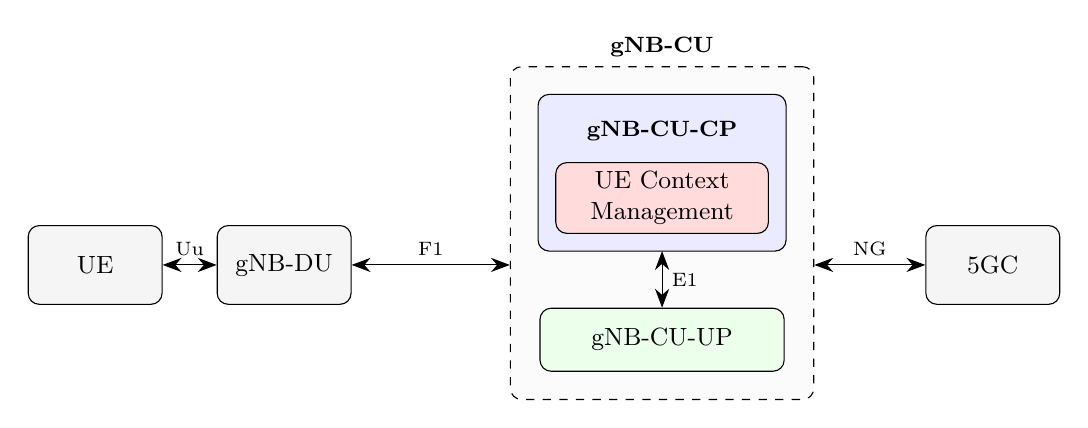
\begin{tikzpicture}[
    font=\small, >={Stealth[length=2.4mm]},
    box/.style={draw, rounded corners, minimum height=1.0cm, minimum width=1.7cm,
                align=center, fill=gray!8},
    cpbox/.style={draw, rounded corners, align=center, fill=blue!8},
    upbox/.style={draw, rounded corners, minimum width=3.1cm, minimum height=0.8cm,
                  align=center, fill=green!8},
    uecm/.style={draw, rounded corners, minimum width=2.7cm, minimum height=0.62cm,
                 fill=red!14, align=center}
  ]
  \node[box] (ue) at (0,0)   {UE};
  \node[box] (du) at (2.4,0) {gNB-DU};

  % Control plane, with UE Context Management shown nested inside it
  \node[font=\footnotesize\bfseries] (cpttl) at (7.2,1.7) {gNB-CU-CP};
  \node[uecm] (uecm) at (7.2,0.85) {UE Context\\ Management};
  % User plane
  \node[upbox] (up) at (7.2,-0.95) {gNB-CU-UP};

  % The background layer paints in source order and the central unit's fill is opaque, so
  % the control-plane box has to be drawn after it. Node (cp) carries the geometry that the
  % central unit and the E1 arrow are measured against.
  \begin{scope}[on background layer]
    \node[fit=(cpttl)(uecm), inner sep=6pt] (cp) {};
    \node[draw, dashed, rounded corners, fill=gray!3,
          fit=(cp)(up), inner sep=10pt, label={[font=\footnotesize\bfseries]above:gNB-CU}] (cu) {};
    \node[cpbox, fit=(cp), inner sep=0pt] {};
  \end{scope}

  \node[box] (core) at (11.4,0) {5GC};

  \draw[<->] (ue) -- node[above,font=\scriptsize]{Uu} (du);
  \draw[<->] (du.east)         -- node[above,font=\scriptsize]{F1} (cu.west |- du);
  \draw[<->] (cu.east |- core) -- node[above,font=\scriptsize]{NG} (core.west);
  \draw[<->] (cp.south) -- node[right,font=\scriptsize]{E1} (up.north);
\end{tikzpicture}
\caption[Where the studied subsystem sits in the 5G NG-RAN]{Where the studied subsystem sits in the 5G NG-RAN. UE Context Management is
highlighted inside the gNB-CU-CP.\label{fig:ngran}}
\end{figure}

\section{Predictability and the two languages}\label{sec:bgbrief}
This section states what the study takes as given.
Predictability, not average
throughput, is the governing property of a latency-critical service, so the quantity to measure
is the tail of the distribution and not its mean, and measuring it correctly
constrains the harness as much as the metric: an open-loop schedule is required, because a
closed-loop one stops issuing requests while a stall is in progress and so never records the
latency of the stall.

C++ supplies the control the domain demands and leaves memory and concurrency safety to the
programmer, with sanitisers and review standing in for a guarantee. The standards committee's
work on enforced safety profiles is neither standardised nor generally implemented. Rust's ownership and borrowing discipline rules out lifetime and
aliasing errors at compile time, and its \texttt{Send} and \texttt{Sync} traits rule out data
races. That is a narrower claim than the phrase ``thread safety'' suggests. It says nothing about
lock-acquisition order, about the atomicity of a composed operation, or about leaks, and it is
suspended wherever a program writes \texttt{unsafe}. Both languages can express the same
concurrency structures, and a comparison that lets the structure vary with the language measures
the structure. The two meet through a C application binary interface, which is the mechanism any
incremental migration has to use and the reason a seam concentrates whatever \texttt{unsafe} a
migration needs.

\section{Research gap}\label{sec:gap}
The preceding sections set up the gap. The RAN control plane is a soft-to-firm real-time,
highly concurrent domain where tail behaviour under overload, not average throughput, governs
the quality the network delivers. C++ supplies the control and performance the domain demands,
but leaves whole classes of memory and concurrency defects to best-effort detection after the
fact. Rust promises to prevent those classes at compile time at no run-time cost, and offers a
credible incremental adoption path through the C application binary interface (ABI).

The domain is not unstudied, and the volume of prior work is easy to underestimate because
almost none of it is indexed. At least five vendor-hosted master's theses, all carried out at
Ericsson, have compared candidate languages for RAN and telecom software. One weighs runtime
cost against development efficiency across C++, Rust, and Go~\cite{karlback2021ran}. One asks
whether Rust could replace C in RAN node management~\cite{olsson2023ranmgmt}. One builds a
thread-per-core packet processor on asynchronous Rust and measures it against the Data Plane
Development Kit (DPDK) application it mirrors~\cite{olsson2023asyncpackets}. One measures median and 99th-percentile
latency for control-plane procedures across five asynchronous programming
frameworks~\cite{arvidsson2025async}. The last builds matched C++ and Rust implementations of an
Abstract Syntax Notation One (ASN.1) decompiler and compares them
statistically~\cite{emberg2023asn1}. All five are directly
relevant, and two report differences unfavourable to Rust.

Three of them vary the language together with the runtime and the concurrency model, so a
measured difference cannot be attributed to the language rather than to the framework built on
it~\cite{karlback2021ran,olsson2023asyncpackets,arvidsson2025async}. The effect sizes reach a
factor of five, which is an indication of how much of the measurement the runtime owns. The
remaining two hold the design closer to fixed but report execution time and peak memory rather
than tail behaviour under rising load~\cite{olsson2023ranmgmt,emberg2023asn1}, and the closest
of them, Emberg and Wadsten, measures a stateless transformation rather than a stateful,
concurrent subsystem. Figure~\ref{fig:gapmap} places the five vendor theses beside the
general-purpose comparisons~\cite{pereira2017energy} and the matched systems-software
pairs~\cite{emmerich2019drivers,suchert2023stamp}. The pattern it shows is that each group holds
some of the properties a controlled answer would need, and none holds all.

The concentration of that evidence is itself part of the gap. All five studies come from one
vendor, and their conclusions have never been tested against another organisation's software,
targets or conventions, so what is known about this question is what one company's frameworks
report about it. The published record on the other side is emptier: there is no study of Rust
among the indexed publications of the vendor hosting this work, and the nearest peer-reviewed
position from that side argues for making memory-error sanitisation practical rather than for
replacing it with a compile-time guarantee~\cite{gjomemo2016mesc}, which is the strategy this
thesis tests against. The paragraphs below compare the five with this study directly.

\begin{figure}[ht]
\centering
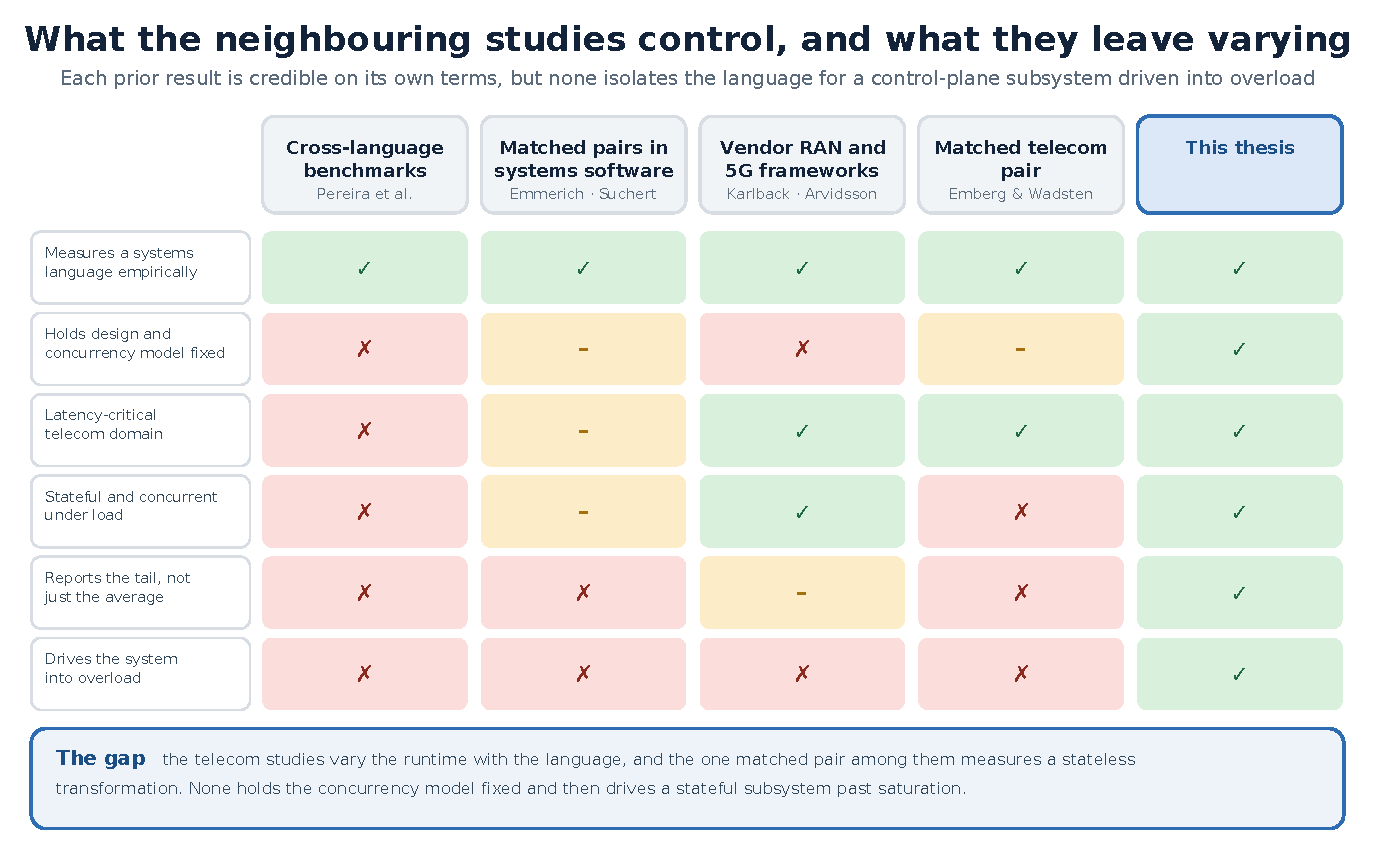
\includegraphics[width=0.78\linewidth]{diagrams/pdf/29_research_gap.pdf}
\caption[What the neighbouring studies control, and what they leave varying]{What the neighbouring studies control, and what they leave varying. Each row is a
property a controlled answer would need, and each column is a group of studies.
The vendor-RAN column is the five Ericsson theses, including both Olsson
studies.\label{fig:gapmap}}
\end{figure}

What is therefore missing from the literature
is \emph{direct, controlled} evidence for a representative control-plane subsystem: Whether
Rust actually holds its tail latency and predictability under overload against modern C++
\emph{when the concurrency model, algorithms, and data structures are held fixed},
exactly which defect classes it eliminates and at what stage the remainder are caught, what
its safety model costs in throughput and resources, and what incremental adoption costs in
practice. Closing this gap is the purpose of the four research questions. The next chapter
grounds them in the specific subsystem, defect classes, and timing properties at stake, and
sets out the methodology by which they are pursued.


\chapter{Research Methodology\label{chapter:methodology}}
\chaptermark{Methodology}

The preceding chapter set out the gap this study closes. This one sets out how.
It begins with the subsystem the work is carried out on. It then states the
research strategy, the method for each question, the controls that keep the
comparison fair, the statistical treatment, and how a third party can rebuild
the results.

\section{The UE Context Management subsystem}\label{sec:uecm}
The subsystem under study is a UE Context Management service. It is modelled on a
real Nokia gNB-CU-CP service domain that owns the UE context lifecycle, RRC
procedure execution~\cite{3gpp38331}, and mobility and handover. Those are the
functions the 3GPP architecture assigns to the control-plane part of a
disaggregated gNB (Section~\ref{sec:ranarch}). Figure~\ref{fig:fsm} shows the
UE-context lifecycle both versions encode the same way. The mixed workload
of Section~\ref{sec:workload} walks each UE through that machine.

\begin{figure}[ht]
\centering
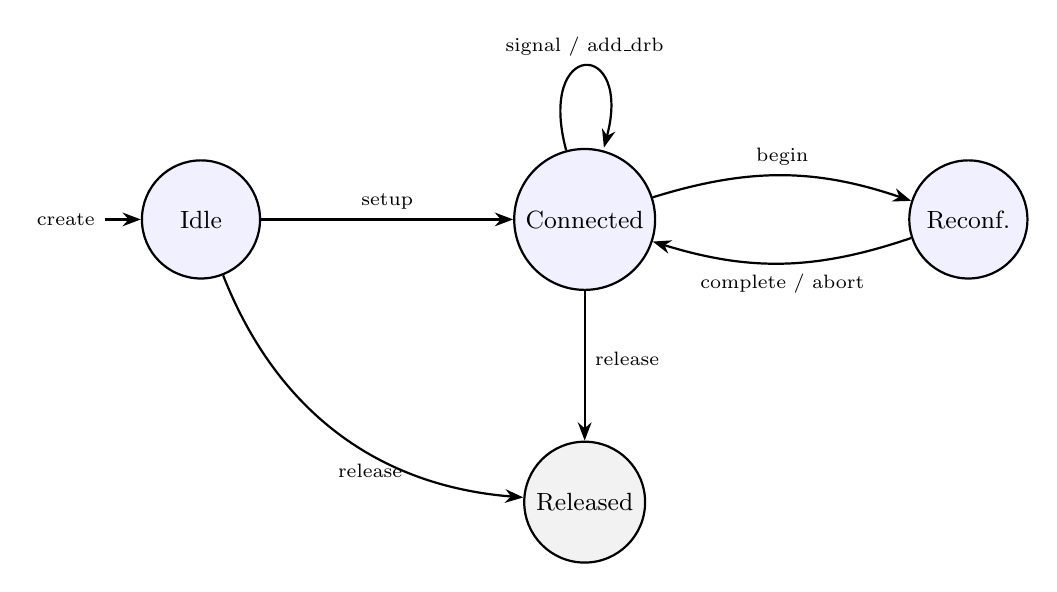
\begin{tikzpicture}[
    ->, >=Stealth, node distance=3.2cm, font=\small,
    every state/.style={draw, minimum size=1.5cm, fill=blue!6, thick},
    every edge/.style={draw, thick}
  ]
  \node[state, initial, initial text=\scriptsize create] (idle) {Idle};
  \node[state, right=of idle] (conn) {Connected};
  \node[state, right=of conn] (reconf) {Reconf.};
  \node[state, below=1.9cm of conn, fill=gray!10] (rel) {Released};

  \path (idle)  edge node[above,font=\scriptsize]{setup} (conn)
        (conn)  edge[bend left=18] node[above,font=\scriptsize]{begin} (reconf)
        (reconf) edge[bend left=18] node[below,font=\scriptsize]{complete / abort} (conn)
        (conn)  edge node[right,font=\scriptsize,pos=0.45]{release} (rel)
        (idle)  edge[bend right=32] node[below,font=\scriptsize,pos=0.6]{release} (rel);
  \path (conn) edge[loop above] node[font=\scriptsize]{signal / add\_drb} (conn);
\end{tikzpicture}
\caption[UE-context lifecycle state machine]{UE-context lifecycle state machine.
Operations invalid for the current state return an error instead of changing
state.\label{fig:fsm}}
\end{figure}

UECM is core RAN layer-3 work. It carries the properties that make
live control-plane code hard: per-UE mutable state, a strict
operation lifecycle, high concurrency across UEs, and the latency targets the 5G
system sets for control-plane procedures~\cite{3gpp38913,3gpp22261}. Conclusions
about how a language handles those properties transfer to other
stateful, concurrent control-plane services. The subsystem is also small enough
to specify in full and implement twice. That is what makes a parity-tested
comparison possible.

The interface is small and built around the lifecycle. It can create and release a
context, set up a connection, handle an in-session signalling message, add a
data radio bearer, begin, complete, or abort a reconfiguration, and look up a
context's state under load. Each operation is defined for each state of
Figure~\ref{fig:fsm}. An illegal operation returns a typed error and leaves the
context unchanged. That closed set lets the same tests and the same workload
drive both versions along the same paths.

RQ2 needs a catalogue, not a loose list of hazards. One is built from this
operation set: $\FaultClasses$ classes in two groups of seven. Seven come from
inside the region safe Rust claims to govern. Seven were chosen because safe
Rust is expected not to prevent them. Each has its expectation recorded before
the programs were run. Section~\ref{sec:safetyresults} reports what each one
did.

The tail is the metric because of two properties of this subsystem. One
user-visible action, a call setup or a handover, becomes many dependent
control-plane operations. The slowest member gates completion. A busy site
drives thousands of such procedures per second, so a percentile far out in the
distribution is reached often enough to matter. The failure shape is the second
reason. A service of this design tracks its offered load with flat latency until
a worker saturates. Then latency jumps by a huge step in one
increment of load. That is why this study sweeps past saturation.

\section{Research approach}\label{sec:approach}
The study runs experiments. It also builds the thing it measures: a matched pair
of versions, plus the harness that drives them. Both are built from one
frozen specification. Evidence comes from three separate methods. A load
sweep answers RQ1 and RQ3. Controlled fault injection answers RQ2. An FFI
migration prototype answers RQ4. A weakness in one of them, such as how
much the host can move the tail, does not carry into the
conclusions as a whole.

Each question asks how one outcome depends on one variable, the
language. The language has to be the only planned gap
between the two objects under test. That rules out the commonest form of
language comparison, where two programs written on their own are measured and
the gap is taken to be the language. Such a gap also carries the design, the
libraries, and the skill of their authors. Building both sides from one
specification removes that confound. Where a question can be answered with
numbers, it uses numbers. Where it cannot, the answer is still by a fixed
plan, in words. That is how this study treats the kind of guarantee in RQ2
and the application programming interface (API) design effort in RQ4.

The closest prior work is the five vendor-hosted theses of
Section~\ref{sec:gap}. They appear in no citation database. They had to be found
by searching the institutional repositories directly. The same searches found no
Finnish thesis on Rust in a radio-access setting, and no indexed publication
mentioning Rust from the vendor hosting this work. The search returned no study
that measures the tail of a Rust and a C++ version of the same stateful,
concurrent control-plane subsystem under overload.

Table~\ref{tab:design} maps each research question to the method, artefact, data
and metric that answer it. RQ1 and RQ3 share H1, worded to cover a speed tie in both the latency
and the resource sense. That wording turns out to be the hypothesis's main
weakness. RQ2 does not depend on the host. RQ4 depends on it along one
axis: build time is a timing, and so it is read as a ratio between two
toolchains measured in turn on one machine.

\begin{table}[ht]
\centering
\small
\caption[How each research question is answered]{How each research question is
answered. RQ1 and RQ3 carry two methods rather than one: the sweep measures the
round-trip a deployment would experience, and the split of the core from the handoff
measures the part of it the language is responsible for.
\label{tab:design}}
\renewcommand{\arraystretch}{1.2}
\setlength{\tabcolsep}{4pt}
\begin{tabular}{@{}p{0.07\linewidth} p{0.27\linewidth} p{0.27\linewidth} p{0.27\linewidth}@{}}
\hline\hline
RQ & Method & Artefact / data & Primary metric \\
\hline
RQ1 & Load sweep to overload, interleaved repeats & Benchmark harness, latency histograms &
median, p99/p99.9/p99.99, and maximum vs.\ offered load \\
RQ3 & Same sweep, resource capture & \texttt{getrusage} samples per run &
peak resident set size (RSS), CPU, throughput \\
RQ1, RQ3 & Core called directly, then through the service &
Matched microbenchmark pair &
operation vs.\ cross-thread handoff \\
RQ2 & Controlled fault injection & Defect catalogue, three C++ sanitisers,
\texttt{rustc}, Loom/Shuttle, Miri &
compile-time / runtime / undetected \\
RQ4 & FFI migration prototype & C++ host $+$ Rust C-ABI seam &
seam size, \texttt{unsafe} scope, per-call cost \\
\hline
\end{tabular}
\end{table}

\section[Methods per research question]{Methods per research question, in outline}\label{sec:methodbrief}
RQ1 and RQ3 are answered by an open-loop load sweep from light load to well past
saturation. Open-loop means the generator keeps to its send schedule instead of
waiting for replies~\cite{schroeder2006openclosed}. The four build variants are
interleaved inside each repeat. A second timing splits the core
operation from the cross-thread handoff around it. The end-to-end round-trip
bundles two costs of two kinds, and only one of them can differ
between the languages. A third timing takes the contended queue and
completion primitives on their own, so the overload cause can be tested
and not merely argued.

RQ2 is answered by controlled fault injection~\cite{natella2016fault}. Each
defect class is written as a small self-contained program in both languages.
The C++ side is built and run under AddressSanitizer, ThreadSanitizer and
UndefinedBehaviorSanitizer. The safe-Rust side is compiled and, where it
compiles, run under a bounded timeout. No static analyser is run, on purpose.
The C++ columns then report the tooling this study ran and not a ceiling on
what C++ tooling could find. RQ4 is answered by a working prototype in the
direction a real migration takes: a C++ host calling an unchanged Rust core
across a C ABI. The per-call cost is measured on a real operation and not
inferred from an empty crossing. Cross-language memory-management defects
concentrate at that seam~\cite{li2022crosslang}.

\section{Fairness as a controlled variable}\label{sec:controlsbrief}
A language comparison is only as good as the variables it holds fixed. The
specification is frozen before either version exists. The concurrency
model, the allocator and its arena count, the optimisation level, the hash
function, the histogram algorithm and the load schedule are matched across the
two sides, never tuned per side. Where the two languages could not be written
alike, the gap is logged instead of resolved. The two sides are shown to
match by diffing conformance transcripts operation by operation. One row
of that table has no control against it: one person wrote both versions
and is not equally expert in both. Section~\ref{sec:standing} treats that as the
study's main internal threat.

\section{Statistical treatment}\label{sec:statsbrief}
The statistical design is fixed in advance. The family of tested comparisons is
listed ahead of the campaign, so a load picked after seeing
a sweep cannot enter it. Each comparison is an exact paired permutation test
over \NRepeats{} interleaved repeats with a bootstrap confidence
interval~\cite{efron1993bootstrap}, Holm-corrected across the
family~\cite{holm1979simple}. The floors the test can reach ($\MinAttainableP$
uncorrected, $\CorrectedFloor$ corrected) are quoted so that a null can be
told apart from a math limit. Two quantities are kept out of the
family. One is jitter from one call to the next, which no research question asks for.
The other is the pooled p99.99 far tail. Its unit is the operation, not the run.
It then has no across-repeat interval to test.

\section{Reproducibility and research artifacts}\label{sec:repro}
A third party can rebuild the results without access to Nokia's private
code. The versions are driven entirely by the public frozen
specification. The benchmarking harness, the fault catalogue and its runner, and
the FFI prototype are published with the thesis. Each plot of measured data,
and each quoted number in the results, is rebuilt by one
script (\texttt{bench/refresh\_thesis.sh}) directly from the raw logs. That
claim does not cover the hand-drawn schematics, which explain a concept rather
than report a result. And running the same scripts over another host's campaign
rebuilds the artefacts by the same procedure, not with the same values.

The logs that script reads are part of the package. Each campaign has its own
script and its own macro prefix, so a figure from one cannot reach a sentence
about another. Each run's host setup is recorded and stored beside the campaign
data. Nothing in the results chapters is transcribed from those files by
hand.

\chapter{Design and Implementation\label{chapter:design}}
\chaptermark{Design}

Nothing is built until the specification is frozen. It fixes the public
API, the UE state machine, the data structures and their algorithms,
the locking and shard grain, and the concurrency model. Both
versions follow it. The test then times the language, not a
gap of design or of skill. The specification is itself a deliverable. It
is the study's main control against writer bias.

One concurrency model is used on both sides, shared-nothing and
thread-per-shard. That structuring is known to change tail latency by
itself~\cite{enberg2019threadpercore}. The identifier space is partitioned into
shards. Each shard is owned by a single worker thread that alone reads or
mutates it, so no lock guards context state. Callers submit a request to the
owning shard's bounded queue and wait on a single-use completion handle. The
queue blocks when it is full. That is deliberate. A drop policy would hide
overload, and this study needs overload to appear as latency. The only shared
mutable state either version permits is one atomic counter. No control flow
depends on its value. Figure~\ref{fig:arch} shows the resulting data flow, with
one multi-producer, single-consumer (MPSC) queue per shard that its worker
drains first in, first out (FIFO).

\begin{figure}[ht]
\centering
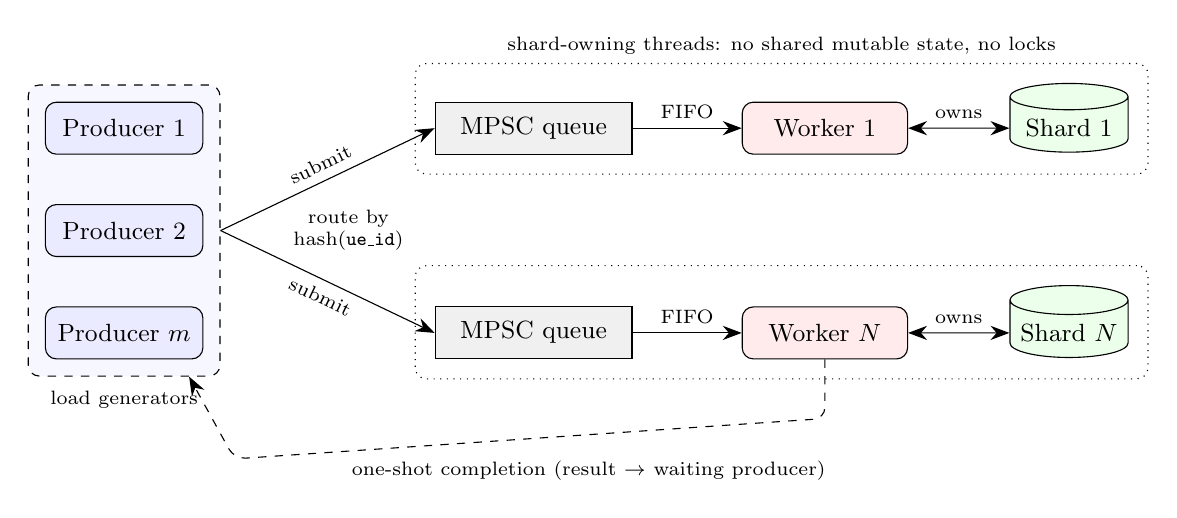
\begin{tikzpicture}[
    font=\small,
    prod/.style={draw, rounded corners, minimum width=2.0cm, minimum height=0.66cm, fill=blue!8},
    queue/.style={draw, minimum width=2.5cm, minimum height=0.66cm, fill=gray!12},
    worker/.style={draw, rounded corners, minimum width=2.1cm, minimum height=0.66cm, fill=red!8},
    store/.style={draw, cylinder, shape border rotate=90, aspect=0.25, minimum width=1.5cm, minimum height=0.85cm, fill=green!8},
    lane/.style={draw, dotted, rounded corners, inner sep=7pt},
    >={Stealth[length=2.4mm]}
  ]
  \node[prod] (p1) at (0,1.3)  {Producer 1};
  \node[prod] (p2) at (0,0.0)  {Producer 2};
  \node[prod] (p3) at (0,-1.3) {Producer $m$};
  \begin{scope}[on background layer]
    \node[draw, dashed, rounded corners, fill=blue!3, fit=(p1)(p2)(p3), inner sep=6pt] (pg) {};
  \end{scope}
  \node[font=\scriptsize] at (0,-2.15) {load generators};

  \node[queue] (q1) at (5.2,1.3)   {MPSC queue};
  \node[worker](w1) at (8.9,1.3)   {Worker 1};
  \node[store] (s1) at (12.0,1.3)  {Shard 1};
  \node[queue] (qn) at (5.2,-1.3)  {MPSC queue};
  \node[worker](wn) at (8.9,-1.3)  {Worker $N$};
  \node[store] (sn) at (12.0,-1.3) {Shard $N$};
  \begin{scope}[on background layer]
    \node[lane, fit=(q1)(s1)] (lane1) {};
    \node[lane, fit=(qn)(sn)] (lanen) {};
  \end{scope}
  \node[font=\scriptsize] at (8.35,2.35) {shard-owning threads: no shared mutable state, no locks};

  \node[font=\scriptsize, align=center, fill=white, inner sep=2pt] at (2.85,0) {route by\\ hash(\texttt{ue\_id})};
  \draw[->] (pg.east) -- (q1.west) node[midway, above, sloped, font=\scriptsize]{submit};
  \draw[->] (pg.east) -- (qn.west) node[midway, below, sloped, font=\scriptsize]{submit};

  \draw[->]  (q1) -- node[above, font=\scriptsize]{FIFO} (w1);
  \draw[->]  (qn) -- node[above, font=\scriptsize]{FIFO} (wn);
  \draw[<->] (w1) -- node[above, font=\scriptsize]{owns} (s1);
  \draw[<->] (wn) -- node[above, font=\scriptsize]{owns} (sn);

  \draw[->, dashed, rounded corners=4pt]
      (wn.south) -- ++(0,-0.75) -- (1.4,-2.9) -- ($(pg.south east)+(-0.4,0)$);
  \node[font=\scriptsize] at (5.9,-3.05) {one-shot completion (result $\rightarrow$ waiting producer)};
\end{tikzpicture}
\caption[Shared-nothing, thread-per-shard architecture]{Shared-nothing,
thread-per-shard architecture. Producers submit to a bounded MPSC queue per
shard, and that shard's worker drains it.\label{fig:arch}}
\end{figure}

Fairness is enforced below the design as well as in it. Both builds link the
same \texttt{jemalloc} and keep a system-allocator build as a control. Both
compile at matched optimisation. Both record latency through one
high-dynamic-range (HDR) histogram algorithm set up the same
way~\cite{tene_hdrhistogram}. Hashing is pinned on both sides, SplitMix64
for shard assignment and FNV-1a, the Fowler--Noll--Vo hash, inside the map.
C++'s default hash of an integer is often just the number itself. Rust's is
strong on purpose. Left as they came, the two standard libraries would
have been the measurement.

Where the languages cannot satisfy a requirement the same way, the gap is
written into a forced-idiom log and then measured. Two of those gaps carry the
overload result of Section~\ref{sec:overload}. One is the bounded queue,
hand-written in C++ against Rust's \texttt{sync\_channel}. The other is the
completion handle, \texttt{std::promise} against a fresh \texttt{mpsc} channel
per request.
A third carries the core-operation result of Section~\ref{sec:perfresults},
since the per-shard container is each language's own standard hash map. Rust
takes its bounded blocking queue from \texttt{sync\_channel}. C++ through C++23
has no such primitive, so it assembles one from a mutex and two condition
variables. C++ has no payload-carrying enumeration in this idiom either. A
request becomes a tagged struct holding each argument field any operation might
need, $\CppRequestBytes$~bytes against Rust's $\RustRequestBytes$. The net
result is a Rust core $\NlocRise\%$ longer in code lines whose total cyclomatic
complexity is $\CcnTotalDrop\%$ lower~\cite{lizard}. The Rust library contains
no \texttt{unsafe} at all.

Parity is tested and not assumed. Language-neutral vectors run in both
versions and their transcripts are diffed operation by operation. A
cross-diff cannot tell ``both correct'' from ``both wrong in the same way''. A
third version in Python acts as an independent oracle. It has to
reproduce all $\ConfHandOps$ hand-derived expectations before it may generate
any of its own. A campaign of roughly $\ConfGenOps$ generated operations found
no divergence. The C++ side runs under AddressSanitizer, ThreadSanitizer and
UndefinedBehaviorSanitizer. The Rust side runs under Miri. A clean sanitiser
result is bounded by the code that actually ran.

\chapter{Experimental Setup and Evaluation\label{chapter:eval}}
\chaptermark{Evaluation}

This chapter starts with the test machines and the workload. The results come
after that, one research question at a time.

\section{Testbed setup\label{sec:testbed}}
Some numbers in this chapter come from the compilers and the code. Other
numbers depend on the computer they ran on. Every speed number here comes from
one dedicated bare-metal server, a single-socket \MainCpu{}. Each core runs one
thread. Simultaneous multithreading is \MainSmt{}. The machine runs
\MainHostDistro{} on kernel \MainKernel{}. Linux can raise and
lower each core's clock as load and temperature change. The clock is held
fixed: the frequency governor is \MainGovernor{}, and boost is off. The
benchmark may use only cores \MainPinned{}. There is no hypervisor, so the
program runs on the machine itself and not inside a virtual machine. On those
cores the kernel turns off its periodic timer interrupt (\texttt{nohz\_full}).
Those interrupts would otherwise appear in the latency numbers. The study does
not use \texttt{isolcpus}. That flag also stops the kernel spreading work
across the allowed cores. Every benchmark thread then lands on one core.

The compilers are not the ones installed on the server. Both versions are built
and run inside a container image that carries \MainDistro{} with
\texttt{g++~\MainGpp} and \texttt{rustc~\MainRustc}. The image pins the
\texttt{gcc-toolset} major version and not the release within it. The earlier
campaign on a virtual machine therefore compiled with \texttt{g++~\GuestGpp},
one GCC~15 release earlier. A container still uses the kernel of the machine
it sits on. The two campaigns then differ in the hardware, in the kernel
(\MainKernel{} against \GuestKernel{}), and in that compiler release.

Until late in the work the campaign ran on a virtual machine instead: a
\GuestCpu{} guest (\GuestVirt{}) with none of the core controls above. On that
host the $95\%$ confidence interval on a single variant's p99 spans
$\GuestPNineNineMaxCI\,\mu$s, while the four variants' p99 values differ by
$\GuestPNineNineRange\,\mu$s. The noise on one variant was larger than the gap
between all four. That campaign is kept. It uses the same design as
this one, so the two can be compared to ask which findings belong to the code.
A third sweep on a second bare-metal \BmCpu{} uses a different shard count, load
grid, repeat count and compilers. It tests whether the findings survive a
change of design rather than a change of machine.

\section[Workload and measurements]{Workload and measurements\label{sec:workload}}
The workload is made for the experiment. The steps it takes come from the 3GPP
rules~\cite{3gpp38401,3gpp38331}. A driver that always sends the same
sequence walks each UE through the connection lifecycle those rules
define. The \emph{signal} workload first connects a set of UEs, then sends the
same signalling operation again and again. That isolates the common path. The
\emph{mixed} workload walks each UE through context creation, setup,
signalling, bearer setup, reconfiguration or handover, and release. A fixed
random order makes both languages see the same counts of each operation kind
for a given seed. That is also a check that the two versions did the same
work. Figure~\ref{fig:workload} shows the two workloads and the sequence the
mixed one walks.

\begin{figure}[ht]
\centering
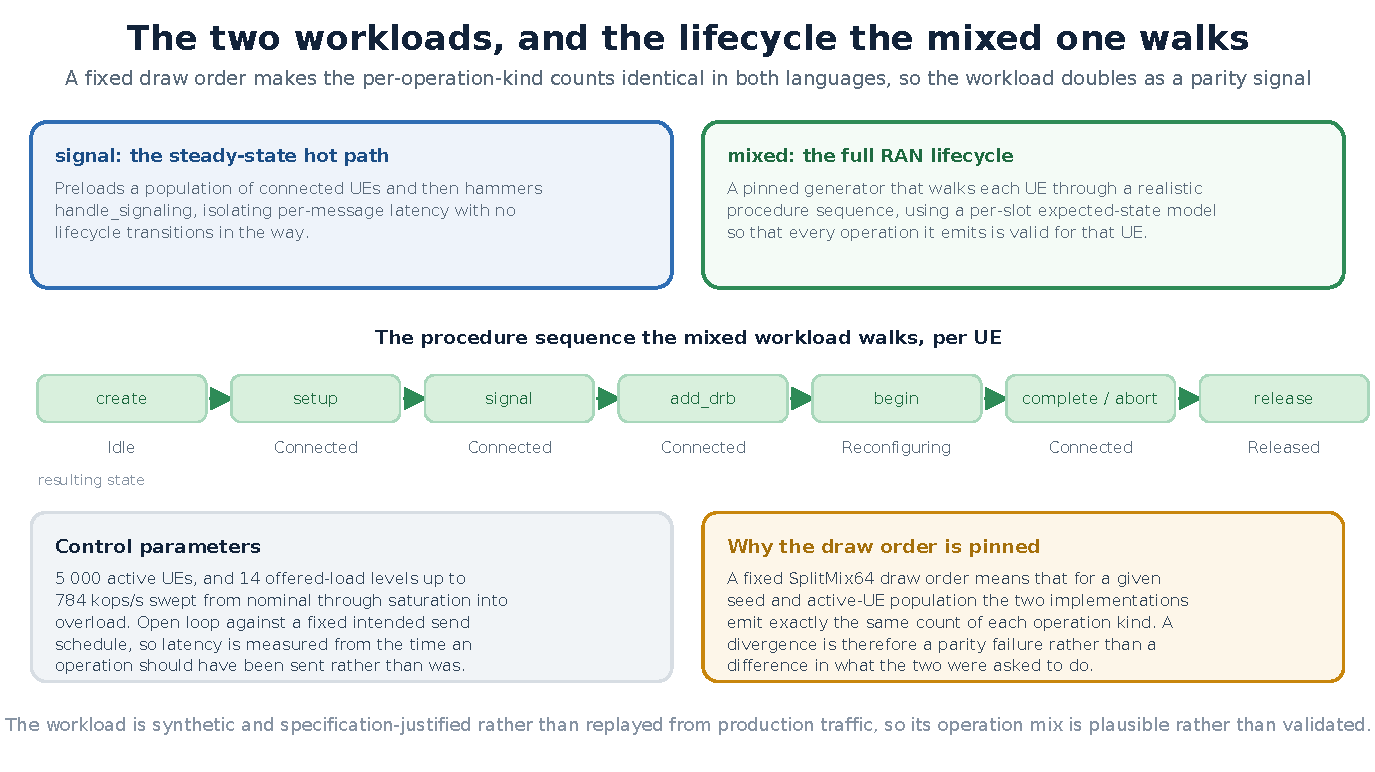
\includegraphics[width=0.78\linewidth]{diagrams/pdf/27_workload_timeline.pdf}
\caption[The two workloads, and the lifecycle the mixed one walks]{The two
workloads, and the lifecycle the mixed one walks. Signal repeats the common
path, and mixed walks each UE through the procedure sequence drawn
below.\label{fig:workload}}
\end{figure}

The sequence of operations matches the 3GPP rules. How often each kind
appears does not. How often a real cell hands over depends on the site and the
time of day, and no public figure fixes it. A mix that does not match a real
cell moves both languages by the same amount. It limits how far the numbers
travel. It does not make the comparison unfair. The sender keeps to its
schedule even if the service is late (open-loop), and the histogram is
corrected, so a stall does not hide missing replies (coordinated-omission
bias)~\cite{schroeder2006openclosed,tene_hdrhistogram}. Each load level is
repeated \NRepeats{} times. The four language and allocator variants take turns
inside each repeat. Each reported point is a median with a bootstrap $95\%$
confidence interval~\cite{georges2007rigorous,efron1993bootstrap}.

The load used for the resource plots is $\ReprLoad$~kops/s. It is a chosen
value, not one computed from the sweep. The first rule this study used was the
busiest load whose p99 stayed under $5$~ms. On the virtual machine that rule
landed on the noise of the host. On a quiet machine it climbs until the service
can no longer keep up. It is kept only as a check. The lowest throughput
plateau among the four variants is $\SatKnee$~kops/s, reached when the offered
load is $\TrackingLoad$~kops/s.

\section{Results}
The safety results and most of the migration results do not depend on which
computer was used. The speed and memory results do. Each figure below was
measured on the host of Section~\ref{sec:testbed} unless the caption says
otherwise.

\subsection{Below saturation (RQ1, RQ3)}\label{sec:perfresults}
When the service still keeps up with the offered load, the four variants'
medians lie within $\PFiftyRange\,\mu$s of each other, $\PFiftySpread\%$. A
paired test still finds a difference of $\PFiftyDiffAbsMax\,\mu$s in Rust's
favour under both allocators. Figure~\ref{fig:loadsweep} shows the sweep behind
that. Higher percentiles can now be read as well. The widest interval on a
single variant's own p99 spans $\PNineNineMaxCI\,\mu$s. The four variants' p99
values differ by $\PNineNineRange\,\mu$s. So the noise on one is smaller than
the gap between them. On the virtual machine the same two quantities were
$\GuestPNineNineMaxCI\,\mu$s against $\GuestPNineNineRange\,\mu$s, the other
way around.

\begin{figure}[ht]
\centering
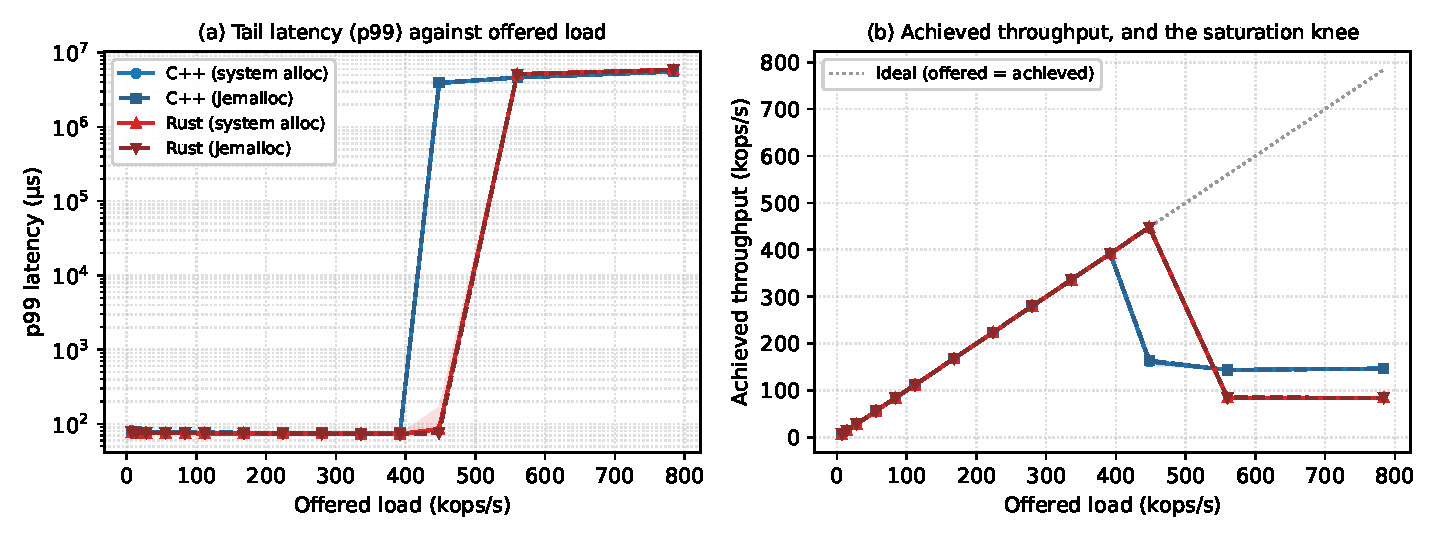
\includegraphics[width=0.78\linewidth]{figures/fig_load_sweep.pdf}
\caption[The load sweep: tail latency and achieved throughput]{The load sweep,
both panels against offered load. Lines are medians over \NRepeats{} repeats,
and the bands are bootstrap $95\%$ confidence intervals.\label{fig:loadsweep}}
\end{figure}

The far tail can be read here too. The repeats' histograms are pooled, which
gives \FarTailSamplesMin{} to \FarTailSamplesMax{} operations per variant. The
two \FarTailLower{} variants sit below the two C++ variants by up to
$\FarTailRange\,\mu$s. A second bare-metal host at another shard count agrees,
running $\BmFarTailCppLo$--$\BmFarTailCppHi\,\mu$s for the C++ variants against
$\BmFarTailRustLo$--$\BmFarTailRustHi\,\mu$s for the Rust ones, with no overlap.
A second limit does not come from the machine. No host would remove it. An
end-to-end round-trip spends only $\BudgetCoreShareMax\%$ of its time on the
work the language performs. The rest is passing the request to another thread,
and that time is charged to the operating system. When the work inside the
language is this small, time spent crossing thread boundaries
dominates~\cite{zhou2025oltp}. This sweep cannot bound a language effect in
either direction, which Figure~\ref{fig:budget} sets beside what the sweep can
still show. Timed on its own, the core operation is $\BudgetCoreRatio\times$
faster in \BudgetCoreFaster{}. The likely cause is how the standard hash map is
laid out, not the safety model.

\begin{figure}[ht]
\centering
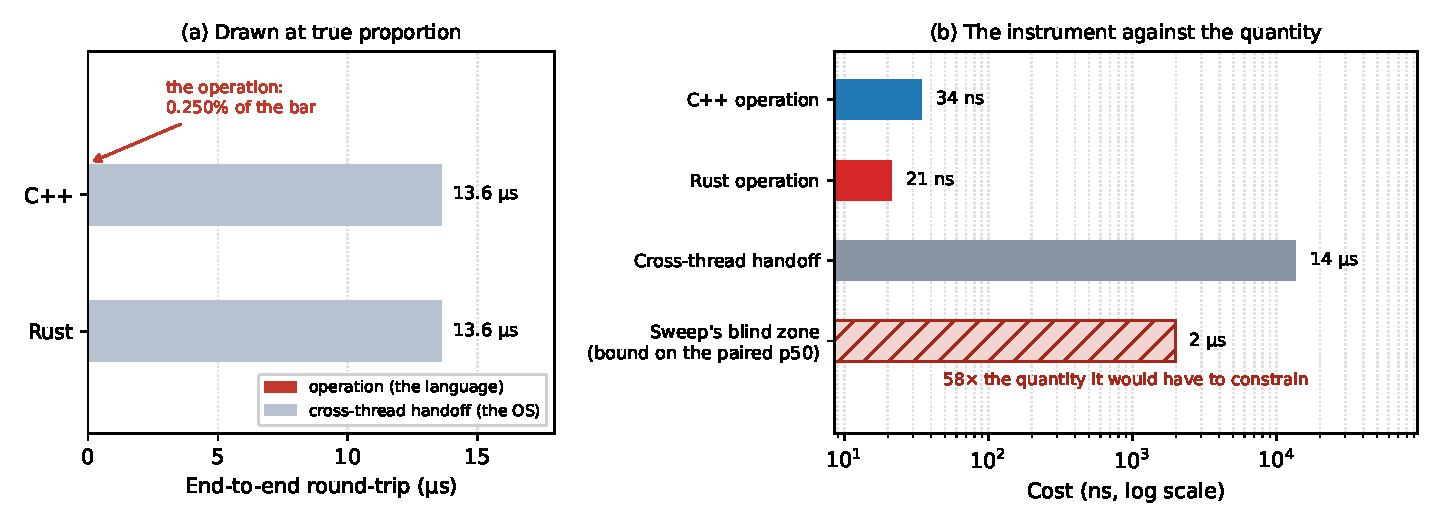
\includegraphics[width=0.78\linewidth]{figures/fig_budget.pdf}
\caption[The end-to-end operation decomposed, against what the sweep can resolve]{Where
an end-to-end round-trip's cost goes. \textbf{(a)} The round-trip at true
proportion. \textbf{(b)} Both operation measurements sit inside the sweep's
blind zone by a factor of $\BudgetBoundVsCore$.\label{fig:budget}}
\end{figure}

\subsection{Past saturation (RQ1)}\label{sec:overload}
Once the offered rate is higher than the service can handle, the four variants
stop keeping up at different loads. The Rust versions hold to
$\TrackingLoadRust$~kops/s. The C++ versions hold to $\TrackingLoadCpp$. So at
$\KneeGapLoad$~kops/s \KneeGapFaster{} still serves $\KneeGapThrFast$~kops/s
where \KneeGapSlower{} has fallen to $\KneeGapThrSlow$. That load level is
described and not tested, because it was found after the data was in hand.

Deeper, at $\OverloadLoad$~kops/s offered, the ordering reverses.
\OverloadSustainedFaster{} still finishes $\OverloadThrCpp$~kops/s where
\OverloadSustainedSlower{} finishes $\OverloadThrRust$, a factor of
$\OverloadThrRatio$, in \OverloadThrAgree{} repeats under both allocators. The
Holm-corrected $p$ is as small as this test family can go. The slower variant
is not simply doing less work. It uses $\OverloadCpuPerOpRatio$ times the CPU
for each operation it finishes, which is the mark of effort spent without
finishing anything. When the bounded queue and the completion handle are
measured by themselves, that ordering is not significant, so the cause sits in
the wider path that passes work between threads. This is the largest language
effect in the tested family. A comparison that stopped at a load the service
still meets would have pointed the other way. Figure~\ref{fig:overload} sets
what each variant still finishes beside what it spends finishing it.

\begin{figure}[ht]
\centering
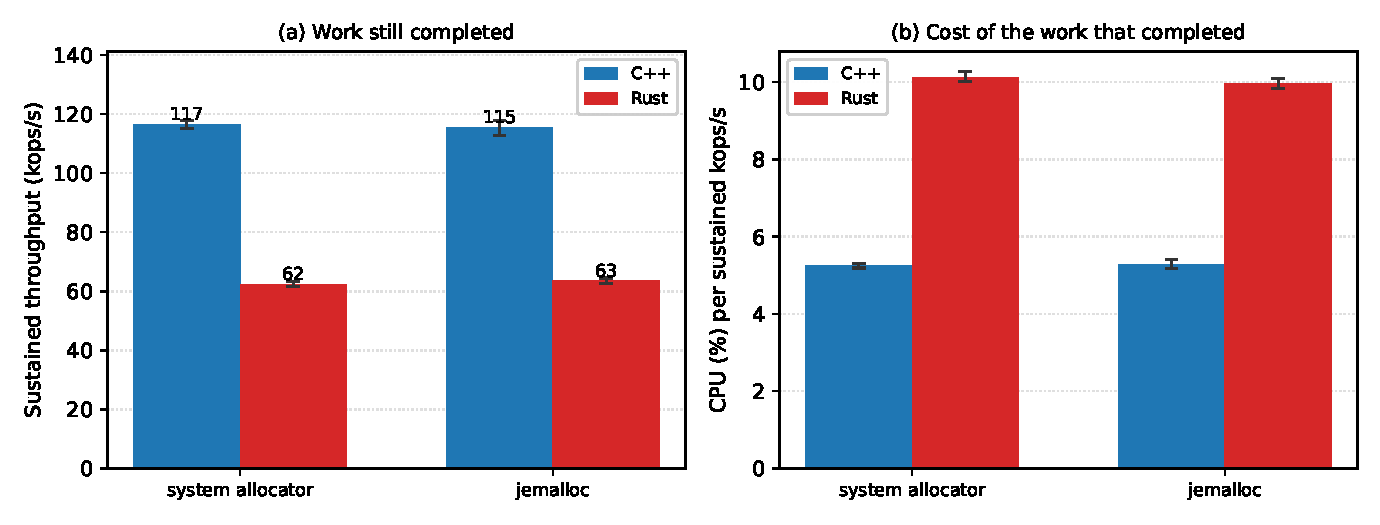
\includegraphics[width=0.78\linewidth]{figures/fig_overload.pdf}
\caption[Divergence past saturation]{Behaviour at $\OverloadLoad$~kops/s
offered. Bars are medians over \NRepeats{} repeats with bootstrap $95\%$
intervals, grouped so the two bars in a group differ only in language. CPU in
(b) is summed across threads.\label{fig:overload}}
\end{figure}

\subsection{Resource use (RQ3)}\label{sec:resources}
Memory and CPU separate the variants where latency could not. Two effects of
similar size sit in peak RSS. The Rust build uses
$\RssLangDiffLo$--$\RssLangDiffHi$~MiB more peak memory than the C++ build
under either allocator. Linking \texttt{jemalloc} at all costs
$\RssAllocDiffLo$--$\RssAllocDiffHi$~MiB in either language. Both are real, and
Figure~\ref{fig:resources} puts the pair beside the peak RSS they add up to.
The language effect keeps its direction and size on all three machines
measured. The allocator's was about ten times larger on the virtual machine
this study used first ($\GuestRssAllocLo$--$\GuestRssAllocHi$~MiB, about
$\GuestRssAllocOverLang$ times the language effect), so their ratio depends on
the machine. The language difference is a fixed cost, not a cost per UE. The
quiet host is where that can be seen. \texttt{jemalloc}'s own counters there
put $\BmJeMetadataDelta$~MiB more in arena bookkeeping and
$\BmJeAllocatedDelta$~MiB \emph{less} in live allocation, and its resident
bytes are $\BmJeResidentDelta$~MiB lower while the process peak is
$\BmJeRssDelta$~MiB higher. The extra memory then sits outside the allocator,
in the runtime a Rust process carries before it allocates. CPU changes sign
with the load. At the representative load of $\ReprLoad$~kops/s Rust uses at
most $\CpuDiffAbsMax$ percentage points less. Once the service no longer keeps
up, CPU per finished operation is much higher.

\begin{figure}[ht]
\centering
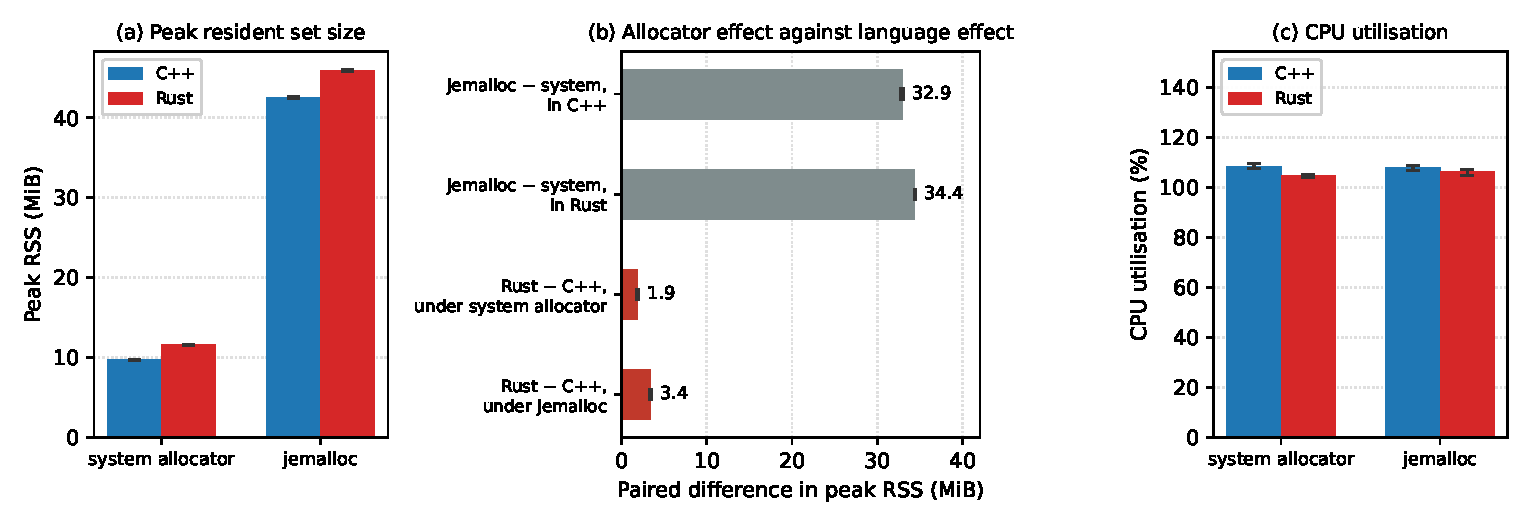
\includegraphics[width=0.78\linewidth]{figures/fig_resources.pdf}
\caption[Resource use, and the two effects inside peak RSS]{Resource use at
$\ReprLoad$~kops/s, grouped by allocator. Bars are medians over \NRepeats{}
repeats with bootstrap $95\%$ intervals, and CPU in (c) is summed across
threads.\label{fig:resources}}
\end{figure}

\subsection{Safety via fault injection (RQ2)}\label{sec:safetyresults}
Safety is measured by injecting $\FaultClasses$ defects. Seven come from inside
the region Rust claims to govern. Seven were chosen because safe Rust is
expected \emph{not} to prevent them. Each one of the first seven is a compile
error in Rust. It cannot be written at all. In C++ each is valid code. The
defect appears only if a test drives it, and no single sanitiser covers them.
The use-after-move is the case where no sanitiser reports anything. A
moved-from object is still a valid object. Its value is unspecified. So there
is nothing illegal to detect, and the identity is simply lost. All seven
boundary cases compile in safe Rust and misbehave. On two of them the C++
tooling is the one that reports. LeakSanitizer flags the reference cycle that
Rust leaks in silence, because leaking is safe in Rust by explicit
design~\cite{hughes2025gcrust,cui2024rcanary}. UndefinedBehaviorSanitizer flags
the overflow that Rust defines to wrap. ThreadSanitizer catches the lock-order
inversion in $\DeadlockTsanHits$ of $\DeadlockTsanRuns$ runs, a rate that is
itself unstable. It records lock orders only from locks that succeed. If the
first inversion waits forever, the cycle is never closed, so the tool never
reports it.

The seam double-free is the in-guarantee double-free rewritten through
\texttt{unsafe}, not a new class. Its C++ half is unchanged, so only the Rust
column moves. Two Rust model checkers do report both original boundary defects.
Loom explores thread interleavings in a sound way. Shuttle samples the ones
Loom cannot reach~\cite{bornholt2021shardstore}. Each had to be written using
the checker's own primitives first, and shrunk to model size. Miri reports the
seam double release, but it interprets Rust and cannot run the C++ host the
defect sits behind. That half of the boundary is caught at test time, and for
the concurrency cases only after a rewrite. Figure~\ref{fig:taxonomy} draws the
whole catalogue as an outcome matrix. Resource Acquisition Is Initialization
(RAII) removes the ordinary missed-unlock. It does not remove the class: both
forgotten-guard programs hang, and neither language's tooling said so.

\begin{figure}[ht]
\centering
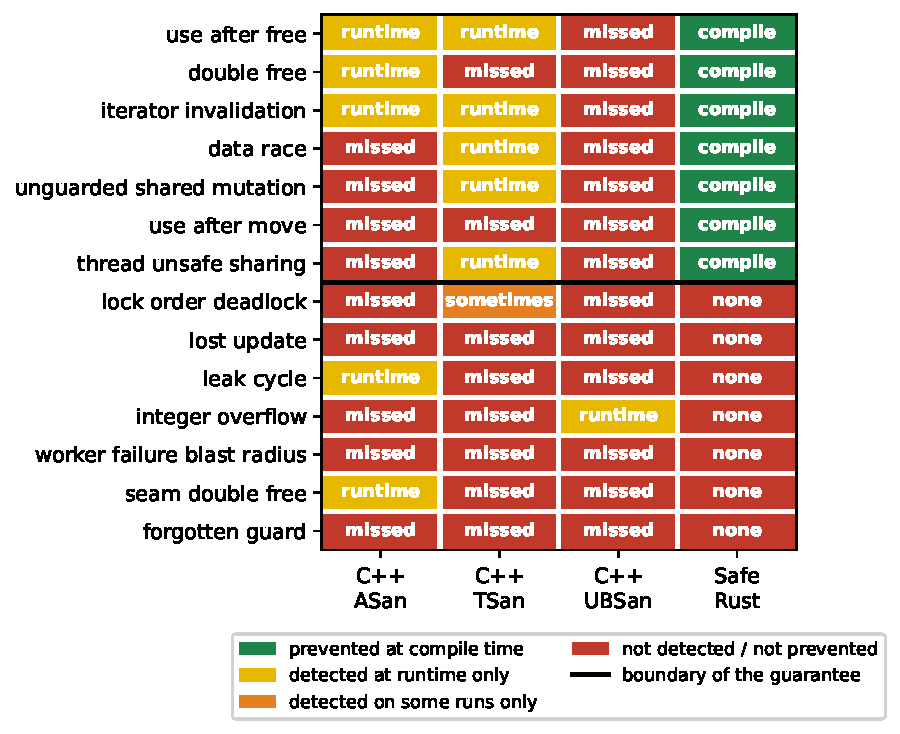
\includegraphics[width=0.72\linewidth]{figures/fig_taxonomy.pdf}
\caption[Where the guarantee stops: the outcome matrix]{The fault-injection
outcomes as a matrix, generated from the taxonomy log.\label{fig:taxonomy}}
\end{figure}

\subsection{Migration (RQ4)}\label{sec:migrationresults}
The migration seam is small on each axis measured: $\FfiEntryPoints$ C entry
points in $\FfiSeamLines$ lines of Rust. All raw-pointer work is confined to
$\FfiUnsafeFns$ functions. The core is left free of \texttt{unsafe}. No extra
cost is detected against the same operation called directly. That bounds any
per-operation tax at $\FfiOpBoundPct\%$ of one operation, and
Figure~\ref{fig:ffiseam} shows the structure that bound belongs to. Three
adoption costs beyond the seam were measured as well, and two of them
contradict the usual objection to adopting Rust.
$\BuildDepShareCpu\%$ of the Rust clean build is third-party code. The project's
own source compiles in $\BuildAllFirstPartyCpuRatio$ times the CPU \texttt{g++}
needs. The $\FootShippedRatio\times$ binary-size gap is a linkage policy that
reverses when the policy is held fixed. The compared component has no
third-party crates and no \texttt{unsafe} sites ($\DepsCore$ crates,
$\CoreUnsafe$ \texttt{unsafe} sites).

\begin{figure}[ht]
\centering
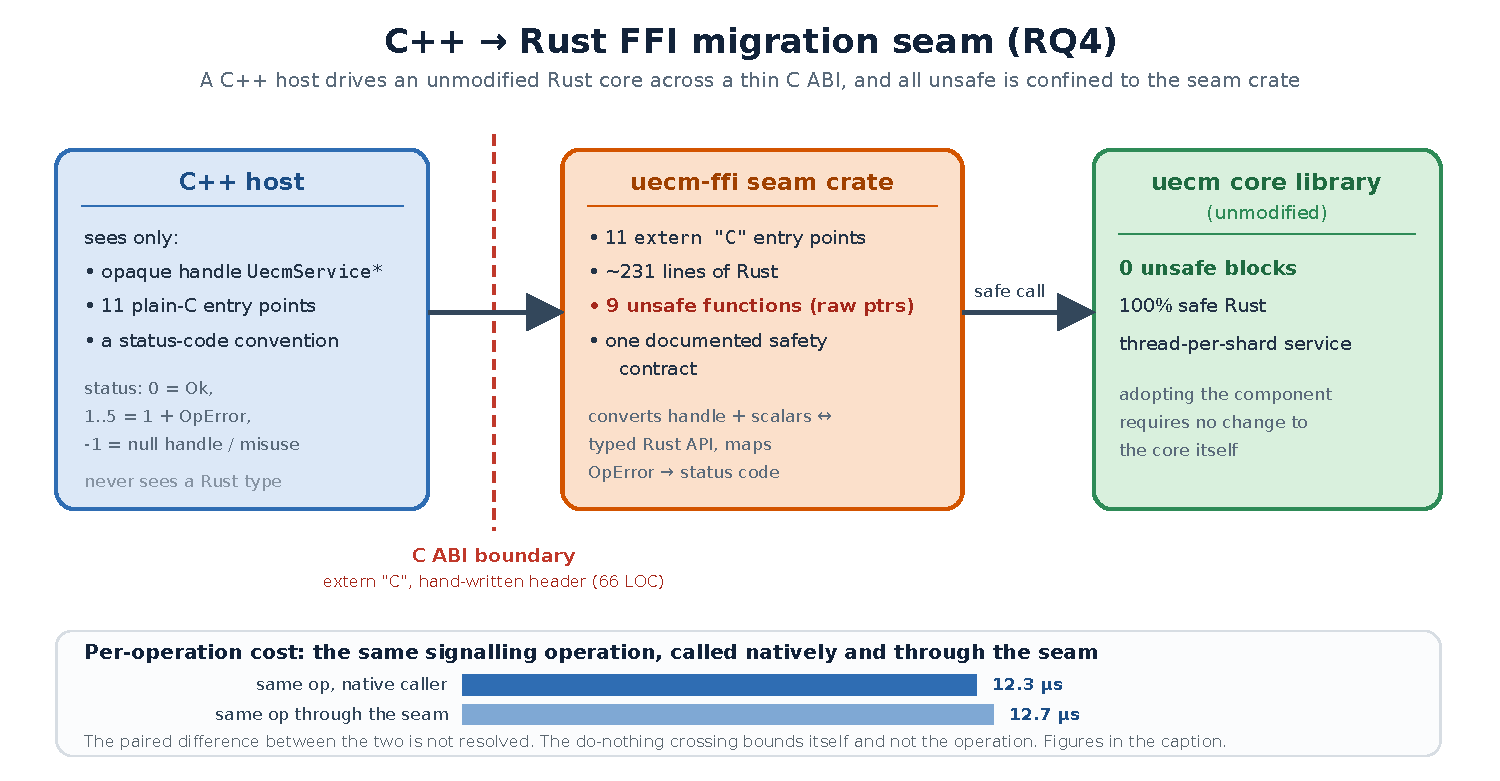
\includegraphics[width=0.78\linewidth]{diagrams/pdf/07_ffi_seam.pdf}
\caption[The C++-to-Rust FFI migration seam]{The C++-to-Rust FFI migration seam.
The same signalling operation costs $\FfiOpNative$~\textmu s directly and
$\FfiOpSeam$~\textmu s through the seam, a paired difference bounded at
$\FfiOpBoundPct\%$ of one operation. A do-nothing crossing costs
$\FfiCrossing$~ns and bounds only itself.\label{fig:ffiseam}}
\end{figure}

\chapter{Discussion\label{chapter:discussion}}

\section{Summary of findings}
The answer to RQ1 divides at saturation. Below it the variants agree to
$\PFiftyRange\,\mu$s at the median, and the far tail resolves in \FarTailLower{}'s favour. The end-to-end round-trip is only $\BudgetCoreShareMax\%$ core operation, so it cannot bound a language effect.
The same operation timed apart is $\BudgetCoreRatio\times$ faster in \BudgetCoreFaster{}. Past saturation they diverge in both directions. The Rust
arms hold their offered rate to $\TrackingLoadRust$~kops/s against
$\TrackingLoadCpp$. At $\OverloadLoad$~kops/s \OverloadSustainedFaster{} sustains $\OverloadThrRatio\times$ the throughput of \OverloadSustainedSlower{}.
RQ2 is final and does not depend on the host. All seven in-guarantee classes are
compile errors in safe Rust. All seven boundary classes compile and
misbehave in both languages. RQ3 is a memory penalty of
$\RssLangDiffLo$--$\RssLangDiffHi$~MiB that reproduces under both allocators and
on all three machines, with CPU that inverts across the two load regimes. RQ4
is a small seam whose per-call tax is bounded at $\FfiOpBoundPct\%$ of one operation. The real
cost is API design and the learning curve.

\section{Discussion on the research questions}\label{sec:rqdiscussion}
What a deployment should do with RQ1 depends on where it expects to sit, not on
a single ranking. A service sized to run below each arm's knee should prefer
the arm that holds its offered rate further. One that a signalling storm will
drive past each knee should prefer the arm that still completes more work
afterwards. Those two preferences point at opposite languages. Only the second
is tested. The first is descriptive, for the reason Section~\ref{sec:overload}
gives. A comparison that stopped at a load the service still meets would have read the
opposite with the same apparatus.

The closest prior work measures this quantity for 5G control-plane procedures.
It finds the same shape and traces it to stackless \texttt{async}/\texttt{await}~\cite{arvidsson2025async}. That attribution is
accepted here. The shape appeared with no asynchronous runtime on either side
and the concurrency model held fixed. A runtime cannot be the only place such an
effect originates. The prediction registered in advance also named where to
look first, bounds and overflow checking~\cite{zhang2022runtime,harris2023morello}.
That part of it was wrong. The median gap is consistent with evidence that
Rust's safety checks are largely absorbed by modern out-of-order
CPUs~\cite{balasubramanian2017rust,emmerich2019drivers}. It is also weaker than
it looks. The core operation is $\BudgetCoreShareMax\%$ of what the sweep
measures.

On safety the difference is one of kind. The boundary is reported as a
first-class result, not as a caveat. A compiler that refuses to build a program
rules the defect out of each execution. A sanitiser rules it out only of the
runs a sanitiser test happens to take. What is absolute there is the
execution coverage, not the breadth of the catalogue.
Figure~\ref{fig:boundary} names the mechanism on each side of that line. Rust
reasons about aliasing and not about acquisition order. A \texttt{Mutex} guard
whose lifetime the borrow checker tracks perfectly says nothing about whether
two threads take their locks in a compatible
order. Static deadlock detection for Rust is an active research
problem~\cite{zhang2026deadlock}. The lost update escapes ThreadSanitizer for the
same reason it escapes the borrow checker. Where each access is correctly
synchronised, there is no unsynchronised access to find. In a field study of
$105$ real concurrency bugs, about a third of the non-deadlock cases violated
the order the programmers intended rather than their
locking~\cite{lu2008mistakes}. Adopting Rust retires one category of concurrency
defect and leaves untouched the category that fails silently. A migration plan
reading ``memory-safe'' as ``concurrency-safe'' would mis-budget its review
effort. Memory-safety bugs in Rust involve \texttt{unsafe} in every published Common
Vulnerabilities and Exposures (CVE) entry but one compiler bug~\cite{xu2021rustcve},
which is why keeping the core \texttt{unsafe}-free matters, and why unsafety
spreading through dependencies is a review concern~\cite{evans2020rust}.

\begin{figure}[ht]
\centering
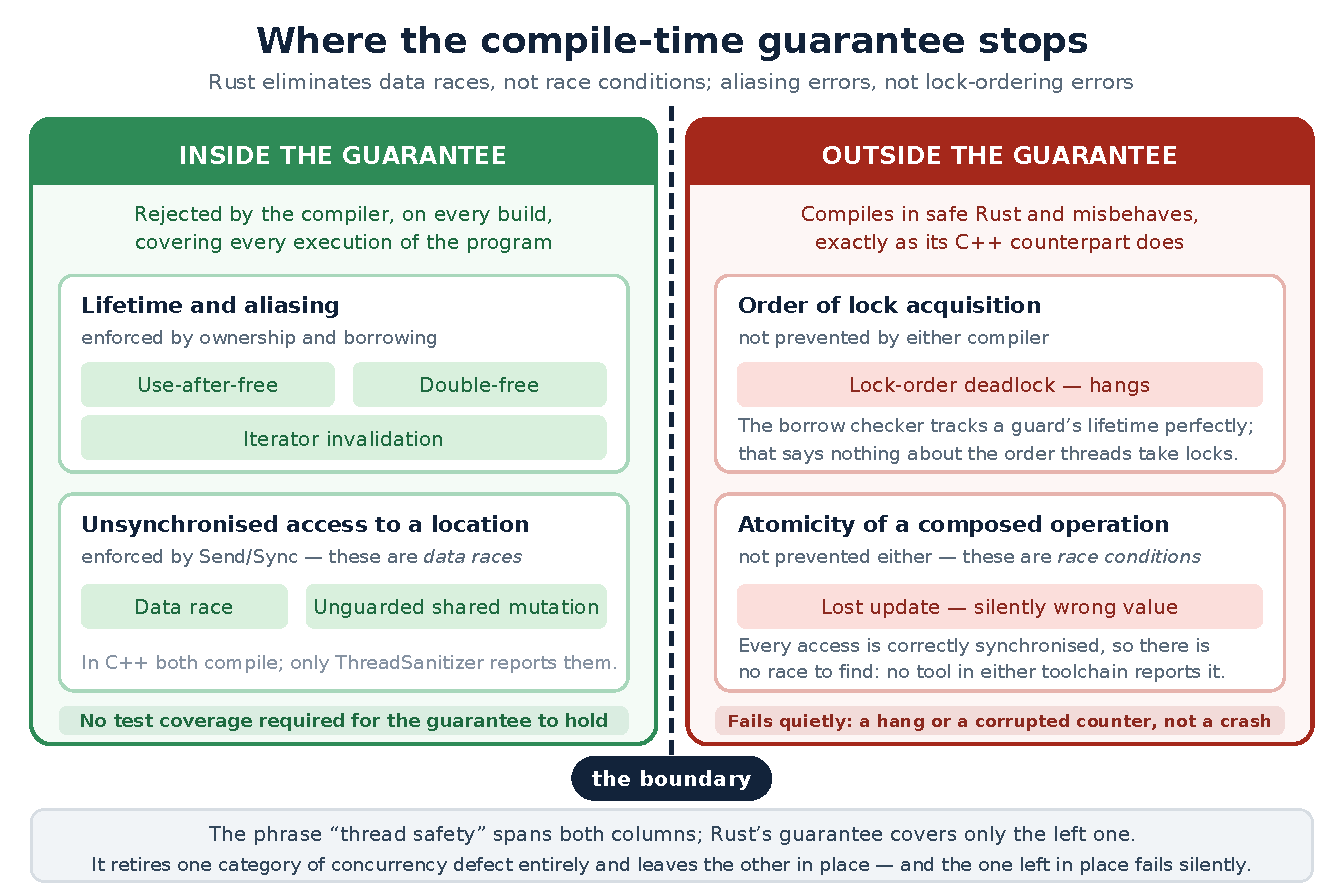
\includegraphics[width=0.78\linewidth]{diagrams/pdf/17_guarantee_boundary.pdf}
\caption[Where Rust's compile-time guarantee stops]{Where Rust's compile-time
guarantee stops, with classes grouped by the mechanism that rejects
them.\label{fig:boundary}}
\end{figure}

One case reaches past the injected programs. A specification gap let an
operation be submitted outside the service's running window. It survived each
test, each parity vector and all three sanitisers because nothing ever called
that path. What turned undefined behaviour into a diagnosable failure on the
Rust side was an ordinary bounds check, not a proof. The property worth
budgeting for is ``checked by default'', not ``ruled out at compile time''. The
root cause belongs to the method. A prohibition stated without a mechanism
behind it leaves each version to fail in its own idiom.

RQ3 splits by resource and the splits do not point the same way. The memory
penalty reproduces under both allocators and on a second machine with a
different compiler. Peak resident set is a run-level maximum, so the jitter that
destroys a p99 does not touch it. Sized against the allocator's own effect, the
two are of the same order on both bare-metal hosts. On the guest the
allocator's was an order of magnitude larger. The language effect travels. The
ratio does not. The quiet host also locates the cost outside the allocator, by
the allocator's own accounting. One close study reports the other way sign, with
Rust lowest and the gap widening as concurrency rises~\cite{karlback2021ran}.
Those two findings agree once the arms are read as two concurrency runtimes.
Their C++ runs on Boost.Fibers, which allocates a stack per fiber. Their Rust
runs on Tokio, where a task is a small heap-allocated future. What they
measured is the per-context cost of two concurrency runtimes.
Two further studies agree with the direction found
here~\cite{olsson2023ranmgmt,sundvisson2026drivers}. On CPU the sign depends on
the load. A single number for ``the CPU cost of Rust's safety model'' would
average two regimes that move in opposite directions.

RQ4 comes out cheap in the machine and expensive in the people. A C++ host can
call an unchanged Rust core across a thin C-ABI seam whose cost on a real
operation is bounded at $\FfiOpBoundPct\%$ of one operation. The dominant cost is
human~\cite{fulton2021adopting,crichton2024learning}. Confining \texttt{unsafe}
to the seam bounds what has to be reviewed, not what can be corrupted. Host and
component share one address
space~\cite{rivera2021galeed,kirth2022pkrusafe}. The build and footprint axes
point the same way as the seam. A vendor worried about either should
audit its dependency budget before blaming the compiler. The one axis where C++
leads outright is the edit-compile loop for changes that stay inside a
translation unit. The $\FootShippedRatio\times$ binary-size figure compares two
linkage policies, and the ordering reverses when the policy is held fixed.

\section{Revisiting the hypotheses}\label{sec:hypotheses}
Section~\ref{sec:rqs} committed to three hypotheses before any measurement.
Stating their disposition is what separates a test from a description.

\begin{description}
  \item[H1] The median clause holds at the representative load. The far-tail
        clause does not, and overload, which the wording never named, is where
        the languages actually part. The reported campaign now resolves that
        tail, in Rust's favour, and a second bare-metal host agrees on the
        direction. H1 was right about where a below-saturation difference would
        show up and wrong that it was the only place. It was also not well
        posed. ``Performance-equivalent'' reads as one quantity and names at
        least three: the delivered round-trip below saturation, the code the
        compilers emit, and sustained work under overload. Those three do not
        move together.
  \item[H2] For the seven injected classes of its kind it holds without
        exception. It fails in the looser reading its wording invites. It is
        accepted for memory safety and data-race freedom, rejected for
        concurrency correctness at large, and it is a claim about \emph{safe}
        Rust only. The seam case shows the same class returning inside
        \texttt{unsafe}.
  \item[H3] Any per-operation tax is bounded at $\FfiOpBoundPct\%$ of one operation, which is
        support from a bound on a cost the measurement could have missed, not
        from the failure to detect one. The accompanying claim, that the real
        cost is design and training, is supported structurally and not
        statistically.
\end{description}

\section{Engineering guidelines for incremental adoption}\label{sec:guidelines}
The guidelines are the practical form of the findings, and each carries the
limit of the finding behind it. Choose a first component for the narrowness of
its interface, not for its size. The redesign of a rich interface is the
schedule risk. The boundary itself is not. Keep the C ABI in its own crate and
the core free of \texttt{unsafe}. That keeps unsafety out of the dependency
chains it otherwise propagates through~\cite{evans2020rust}. Leave the
concurrency review budget where it is. Prefer a shared-nothing structure in
either language. The strongest concurrency result here belongs to the design and
to neither compiler. Plan the learning curve as a training cost and instrument
it. Measure the component as well as the round-trip. Sweep past the point where
the service stops coping. That is the guideline this study would most like to
have followed from the start.

\section[Where this study sits]{Where this study sits, and what it cannot support}\label{sec:standing}
The studies closest to this one are the five vendor-hosted theses of
Section~\ref{sec:gap}. Their verdicts contradict each other in each direction.
The one reporting the other way sign on peak memory reconciles with this study
once its arms are read as two concurrency runtimes rather than two languages.
Three threats stay load-bearing, and the first is that one author wrote both
versions. The same failure mode reversed a published verdict in this
industry: comparable after a code review and then Rust worse by $85$--$91\%$
after further optimisation~\cite{emberg2023asn1}. The parity suite bounds
behaviour and not performance. The end-to-end instrument measures the design
faithfully and the language barely at all. The overload divergence is replicated
here with its mechanism narrowed and not closed, and no peer-reviewed study
reports the same reversal.

\section{Ethical and professional reflection}
The study processes no personal, subscriber, or operator-confidential data. All
traffic is synthetic and the subsystem is modelled on live code rather
than copied from it, so the artefacts can be released openly. The first
responsibility is not to over-claim. A vendor could read the RQ2 result as
licence to describe a migrated component as ``safe'', and the boundary cases are
why that reading would be wrong. A deadlocked control plane is an outage. A
silently lost counter update can misinform a mobility decision. Nothing
demonstrated here prevents either. The second responsibility is how far the
evidence reaches. Tail-latency numbers from any single machine are a narrower
basis for a production commitment than they look. That is why the earlier
guest campaign is reported rather than discarded.

\chapter{Conclusion and Future Work\label{chapter:conclusions}}

The thesis compared modern C++ and Rust. The object is a UE Context Management
service modelled on a real Nokia gNB-CU-CP component. It looked at four dimensions:
tail-latency predictability, compile-time defect prevention, safety-model
overhead, and cost of adding Rust a piece at a time. Both versions were built against
one frozen specification and driven along the same code paths. That is what
lets a language effect be told apart from a difference of design or of skill.

On safety the difference is one of kind and it has a clear boundary. Safe Rust
rejects all seven injected memory-safety and data-race classes at compile time.
Hazards that C++ can only hope to catch under a sanitiser test become programs
that cannot be written. All seven boundary classes compile and misbehave in safe
Rust as they do in C++. On two of them the C++ tooling reports what Rust's does
not. Stated precisely, Rust eliminates data races and aliasing errors. It does
not eliminate race conditions, lock-ordering errors, leaks, wrapping arithmetic
or the blast radius of a failed worker, and it eliminates nothing inside an \texttt{unsafe} block.
Where the boundary defects are caught, they are caught at test time. In two of
the three cases that happens only after the defect is rewritten into a model
checker's primitives.

On migration the cost is dominated by API design and the learning curve, not by
any run-time tax. An unchanged Rust core can be driven from C++ across a thin
seam. The cost on a real operation is bounded at $\FfiOpBoundPct\%$ of one operation.
All of the \texttt{unsafe} sits in the seam, and the core is verified free of it.
Most of the Rust build's extra expense is compiling dependencies, not the
compiler's own work. The binary-size gap is a linkage policy. The ordering
depends on which matched policy is chosen. Where C++ leads is the edit-compile
loop, and it leads only for edits that stay inside a translation unit.

On performance the evidence first divides by what is being measured. An
end-to-end round-trip here is $\BudgetCoreShareMax\%$ language. The rest is an
operating-system handoff. An end-to-end null bounds nothing about either
compiler. The same operation measured apart is $\BudgetCoreRatio\times$ faster
in \BudgetCoreFaster{}. At the fixed load the paired test resolves
$\PFiftyDiffAbsMax\,\mu$s in Rust's favour, too small for a deployment to care
about at the median. At p99.99 the slowest Rust variant sits
$\FarTailLangSep\,\mu$s below the fastest C++ one. The Rust arms then hold their
offered rate to $\TrackingLoadRust$~kops/s against $\TrackingLoadCpp$. Once all
four have collapsed, \OverloadSustainedFaster{} sustains $\OverloadThrRatio\times$
the throughput of \OverloadSustainedSlower{}, which spends
$\OverloadCpuPerOpRatio\times$ the CPU on each operation it completes. On memory
the Rust build carries a few MiB more fixed footprint under both allocators, in
the same direction and scale on all three machines measured. The
allocator choice costs about as much on both bare-metal hosts, and an order of
magnitude more on the guest this study used first.

Taken together these support a narrow claim. It is for stateful, concurrent,
partitionable control-plane services of this kind. At the loads where the
service still meets its offered rate, the choice is which classes of defect a
team wants to make unwriteable. The other half is whether it will pay the
design and training cost of getting them. Past that point it is a speed
decision as well. What the thesis adds is an instrument, not a verdict. That
instrument is the frozen specification and the parity-tested pair. It is also a
timing framework that reaches past the saturation knee. A split of the
round-trip says how much of what it times the language can own. A defect
catalogue maps where the guarantee stops.

Future work answers the gaps one at a time. The first job needs
no new machine: vary the transparent-hugepage policy on one host with everything
else held fixed. All three hosts agree that the Rust build carries the larger
footprint. They disagree about how that compares against the cost of the
allocator. The guest put it an order of magnitude higher, and neither
bare-metal host does. The hugepage policy is the candidate this study
can name but not test, because it differed between the hosts and only the
system-allocator arm inherits it. Beyond that, replaying anonymised production
traces would check the operation mix. The framework can also take further
control-plane subsystems or the data-heavy layer-2 and physical layer (PHY)
path. A subsystem with truly shared mutable state would exercise the two
languages differently than a shared-nothing design does. Testing Rust async runtimes against the thread-per-shard model
would separate the runtime from the language in the tail
result~\cite{arvidsson2025async}. Timing what in-process isolation of the two
heaps costs would price what protecting an \texttt{unsafe}-free core is
worth~\cite{rivera2021galeed,kirth2022pkrusafe}. A longer case study tracking
defect counts and review effort while adding Rust a piece at a time is what would
settle the human cost this study can only name.

% Declaration of generative-AI use, required by the University when a language model has
% been used. Shared with Ha_Vien_Mastersthesis_2026.tex: edit ai_statement.tex, not a copy.
%% Declaration of generative-AI use. The University of Helsinki requires a student who
%% has used a language model in preparing a thesis to state in writing which model was
%% used and in what way; the model may not be named as an author or cited as a source.
%%
%% Shared verbatim by Thesis_POC.tex and Thesis_v1.tex so the two cannot drift apart.
%% It uses no generated macros and no chapter numbers, because the two documents number
%% their chapters differently.
%%
%% The order of the paragraphs follows the University's basic reporting instruction:
%% what the use covered, what it was for, which tool, how it performed and how its
%% output was checked, and what the author took from it.

\cleardoublepage
\phantomsection
\addcontentsline{toc}{chapter}{Statement on the Use of AI Tools}
\chapter*{Statement on the Use of AI Tools}
\markboth{Statement on the Use of AI Tools}{Statement on the Use of AI Tools}

\noindent\textbf{Tool.} Anthropic's Claude Opus~5, used through the Cursor development
environment, is the only generative AI system used in the preparation of this thesis. It was
used throughout the work, from June to August~2026. Following University of Helsinki policy the
model is neither named as an author nor cited as a source: it cannot take responsibility for
what it produces, and it cannot reliably vouch for the literature it paraphrases.

\noindent\textbf{What the assistance covered.} It was extensive, and is declared as such. The
model drafted and revised the running prose of this thesis and proposed the order in which its
arguments are made. It wrote and refactored the two implementations of the UE Context
Management service, the load generator, the fault-injection catalogue, and the interoperability
prototype. It wrote the analysis code behind the bootstrap confidence intervals, the exact
paired permutation tests, and the Holm correction, together with the figure-generating and
build scripts and the \LaTeX{} sources. It also suggested candidate literature.
% ==================== ACTION REQUIRED BEFORE SUBMISSION ==========================
% The abstract of Thesis_POC.tex was drafted with model assistance. The University's
% thesis guide states that a language model may not be used when preparing the thesis
% summary, and in this programme the summary also serves as the maturity test, where
% AI use is never permitted. Rewrite the abstract unaided before submitting; until
% that is done the closing sentence of this paragraph is not yet true of Thesis_POC.
% =================================================================================
The abstract was written by the author unaided, as the University's thesis guide requires of
the thesis summary.

\noindent\textbf{What the model did not settle.} The research problem, the four research
questions, and the three hypotheses are the author's, as is the control on which the study's
value rests: freezing one language-neutral specification and one concurrency model, so that the
language remains the only systematic difference between the two implementations. So is the
decision that keeps RQ2 falsifiable, namely to carry two defect classes -- a lock-order deadlock
and a lost update -- that lie outside Rust's compile-time guarantee and can therefore embarrass
the premise rather than confirm it. Every measurement reported here was run by the author on the
hosts documented in this thesis; no measured value came from a language model. Each measured
number reaches the text through a macro regenerated from the raw logs, so a figure cannot be
transcribed by hand, by the author or by the model. The readings of those numbers are the
author's as well, including the two restraints the evidence imposes: that a far tail a
virtualised host cannot resolve must not be reported as equivalence, and that a sweep dominated
by cross-thread handoff cannot bound an effect of the language.

\noindent\textbf{How the output was checked.} Model output was treated as a draft to be
falsified rather than as a result. Claims were checked against the sources cited for them: every
bibliography entry was resolved against Crossref, DataCite, or the issuing body, and each was
traced to the page or clause carrying the claim made of it. That audit found four passages where
the prose overstated or misplaced its source, one of them a sentence inside quotation marks that
does not appear in the work it was attributed to; all four were corrected, and the audit is kept
with the artefacts so that the correction remains reviewable. Code was checked by running it:
the two implementations are held to one conformance suite whose transcripts are diffed line by
line, and the fault catalogue fixes the expected outcome of each defect before it is injected,
so that a surprise appears as a discrepancy instead of being explained away afterwards. Nothing
is asserted here on the model's authority.

\noindent\textbf{What the author took from it.} The model is dependable at mechanical work --
transposing an idiom between two languages, restructuring a table, keeping a build honest -- and
undependable in a specific and predictable way: it will supply a plausible citation for a claim,
a plausible cause for a measurement, and a confident sentence where the data supports a hedge.
Its fluency is not evidence. The lasting lesson of the work was accordingly less about either
language than about verification. The effort saved in drafting is spent again, and rightly, in
checking, and the parts of this thesis that are defensible are the parts that were checked
against a source, a specification, or a measurement.

\noindent\textbf{Responsibility.} The author is responsible for the whole of this thesis: its
language, its facts, its code, its measurements, and its conclusions. Where it is wrong, the
error is the author's.


% STEP 5:
% The bibliography style is selected with the biblatex options in the preamble.

\cleardoublepage %fixes the position of bibliography in bookmarks
\phantomsection

\addcontentsline{toc}{chapter}{\bibname} % This lines adds the bibliography to the ToC
\printbibliography

\end{document}
